\documentclass[12pt,a4paper]{report}

% ======================================================================
% PACKAGES
% ======================================================================
\usepackage[utf8]{inputenc}
\usepackage[T1]{fontenc}
\usepackage{graphicx}
\usepackage{float}
\usepackage{geometry}
\usepackage[table,dvipsnames]{xcolor}
\usepackage{fancyhdr}
\usepackage{titlesec}
\usepackage{hyperref}
\usepackage{booktabs}
\usepackage{tabularx}
\usepackage{longtable}
\usepackage[most]{tcolorbox}
\usepackage{amsmath}
\usepackage{listings}
\usepackage{enumitem}
\usepackage{setspace}
\usepackage{tikz}
\usepackage{caption}
\usepackage{microtype}
\usepackage{lmodern}
\usepackage{array}
\usepackage{colortbl}
\usepackage{multirow}
\usepackage{parskip}
\usepackage[section]{placeins}

\usetikzlibrary{
  shapes.geometric,
  arrows.meta,
  positioning,
  fit,
  backgrounds,
  calc,
  shadows
}

% ======================================================================
% COLOURS
% ======================================================================
\definecolor{Cream}{HTML}{FFF8EA}
\definecolor{LightCream}{HTML}{FFFDF7}
\definecolor{MutedRose}{HTML}{9E7676}
\definecolor{DeepRose}{HTML}{815B5B}
\definecolor{DarkEarth}{HTML}{594545}
\definecolor{CodeBg}{HTML}{F7F3EF}
\definecolor{ShadowGray}{HTML}{CCBBBB}
\definecolor{AMint}{HTML}{5B8178}
\definecolor{ABlue}{HTML}{5B6F81}
\definecolor{AAmber}{HTML}{A87C45}
\definecolor{LightBorder}{HTML}{E8D5C8}

% ======================================================================
% PAGE GEOMETRY
% ======================================================================
\geometry{
  a4paper,
  top=2.5cm, bottom=2.8cm,
  left=2.8cm, right=2.4cm,
  headheight=24pt, headsep=0.6cm,
  footskip=1.2cm
}

\setstretch{1.25}
\setlength{\parskip}{6pt}
\setlength{\parindent}{0pt}

% ======================================================================
% SECTION FORMATTING
% ======================================================================
% Chapter: hang style — number and title on the SAME line, no negative sep, no TikZ inline
\titleformat{\chapter}[hang]
  {\normalfont\sffamily\huge\bfseries\color{DarkEarth}}
  {\textcolor{DeepRose}{\rule[-6pt]{5pt}{28pt}}\hspace{14pt}%
   \textcolor{DeepRose}{\thechapter}\hspace{14pt}%
   \textcolor{LightBorder}{\rule[-6pt]{1.5pt}{28pt}}\hspace{14pt}}
  {0pt}
  {}
  [\vspace{6pt}{\color{MutedRose}\rule{\linewidth}{0.8pt}}\vspace{8pt}]
\titlespacing*{\chapter}{0pt}{30pt}{18pt}

\titleformat{\section}
  {\normalfont\sffamily\Large\bfseries\color{DeepRose}}
  {\thesection}{0.8em}{}
  [\vspace{-4pt}\color{LightBorder}\rule{\linewidth}{0.6pt}]

\titleformat{\subsection}
  {\normalfont\sffamily\large\bfseries\color{DarkEarth}}
  {\thesubsection}{0.8em}{}

\titleformat{\subsubsection}
  {\normalfont\sffamily\normalsize\bfseries\color{MutedRose}}
  {\thesubsubsection}{0.8em}{}

% ======================================================================
% HEADER & FOOTER
% ======================================================================
\pagestyle{fancy}
\fancyhf{}
\renewcommand{\headrulewidth}{0.6pt}
\renewcommand{\footrulewidth}{0.4pt}
% Left: fixed brand name — never overflows
\fancyhead[L]{\textcolor{DarkEarth}{\sffamily\small\bfseries DokuMind}}
% Right: current section (shorter than full chapter name), no-uppercase
\fancyhead[R]{\textcolor{MutedRose}{\sffamily\small\nouppercase{\rightmark}}}
\fancyfoot[C]{\textcolor{DarkEarth}{\sffamily\small\thepage}}
\renewcommand{\headrule}{{\color{MutedRose}\hrule width\headwidth height\headrulewidth\vskip-\headrulewidth}}
\renewcommand{\footrule}{{\color{MutedRose}\hrule width\headwidth height\footrulewidth\vskip-\footrulewidth}}

% Chapter-opening pages (LaTeX auto-resets them to 'plain') — clean footer only
\fancypagestyle{plain}{
  \fancyhf{}
  \renewcommand{\headrulewidth}{0pt}
  \renewcommand{\footrulewidth}{0pt}
  \fancyfoot[C]{\textcolor{DarkEarth}{\sffamily\small\thepage}}
}


% ======================================================================
% TCOLORBOX ENVIRONMENTS
% ======================================================================
\newtcolorbox{conceptbox}[2][]{
  enhanced, colback=Cream, colframe=DeepRose, coltitle=white,
  fonttitle=\sffamily\bfseries, title={#2},
  attach boxed title to top left={yshift=-2mm,xshift=8mm},
  boxed title style={colback=DeepRose,colframe=DeepRose,rounded corners},
  arc=4pt, boxrule=0.8pt, left=8pt, right=8pt, top=10pt, bottom=8pt, #1
}
\newtcolorbox{infobox}[1][]{
  enhanced, colback=ABlue!8, colframe=ABlue!50,
  arc=3pt, boxrule=0.6pt, left=8pt, right=8pt, top=6pt, bottom=6pt, #1
}
\newtcolorbox{warningbox}[1][]{
  enhanced, colback=AAmber!10, colframe=AAmber!60,
  arc=3pt, boxrule=0.6pt, left=8pt, right=8pt, top=6pt, bottom=6pt, #1
}
\newtcolorbox{techbox}[2][]{
  enhanced, colback=CodeBg, colframe=MutedRose!60, coltitle=DarkEarth,
  fonttitle=\sffamily\small\bfseries, title={#2},
  arc=3pt, boxrule=0.6pt, left=6pt, right=6pt, top=6pt, bottom=6pt, #1
}

% ======================================================================
% CODE LISTINGS
% ======================================================================
\lstdefinestyle{dokustyle}{
  backgroundcolor=\color{CodeBg},
  commentstyle=\color{MutedRose}\itshape,
  keywordstyle=\color{DeepRose}\bfseries,
  numberstyle=\tiny\color{ShadowGray},
  stringstyle=\color{AMint},
  basicstyle=\ttfamily\small\color{DarkEarth},
  breaklines=true, captionpos=b, keepspaces=true,
  numbers=left, numbersep=8pt,
  frame=single, rulecolor=\color{LightBorder},
  xleftmargin=16pt, framexleftmargin=8pt,
  tabsize=2
}
\lstset{style=dokustyle}

% ======================================================================
% HYPERREF
% ======================================================================
\hypersetup{
  colorlinks=true, linkcolor=DeepRose,
  urlcolor=ABlue, citecolor=DarkEarth,
  pdftitle={DokuMind Enterprise - Full Technical Report},
}

% ======================================================================
% TIKZ STYLES  — safe, no-overlap defaults
% ======================================================================
\tikzset{
  % Service box: fixed width, auto height
  svc/.style={
    rectangle, rounded corners=5pt,
    draw=#1!70, fill=#1!12,
    text width=2.4cm, minimum height=1cm,
    align=center, font=\sffamily\scriptsize\bfseries
  },
  % Database cylinder
  dbs/.style={
    cylinder, shape border rotate=90, aspect=0.25,
    draw=#1!70, fill=#1!15,
    text width=1.8cm, minimum height=0.9cm,
    align=center, font=\sffamily\scriptsize\bfseries
  },
  % Generic process box
  proc/.style={
    rectangle, rounded corners=3pt,
    draw=#1!60, fill=#1!10,
    text width=2.6cm, minimum height=0.9cm,
    align=center, font=\sffamily\scriptsize\bfseries
  },
  % Decision diamond
  dec/.style={
    diamond, aspect=2.0,
    draw=AAmber!70, fill=AAmber!12,
    text width=1.6cm, minimum height=0.7cm,
    align=center, font=\sffamily\scriptsize\bfseries
  },
  % Arrow
  arr/.style={
    -{Stealth[length=5pt,width=3.5pt]},
    line width=1pt, color=#1
  },
  % Edge label
  lbl/.style={font=\sffamily\scriptsize, color=DarkEarth, align=center},
  % Dashed group outline
  grp/.style={
    rectangle, rounded corners=6pt,
    draw=#1!45, fill=#1!5,
    dashed, line width=0.8pt
  }
}

% ======================================================================
\begin{document}
% Prevent text from overflowing into margins anywhere in the document
\sloppy
\setlength{\emergencystretch}{2em}

% ======================================================================

% ==============================================================
% PAGE DE GARDE  — Clean professional cover page
% ==============================================================
\begin{titlepage}
\pagecolor{LightCream}

% Top solid colour band
\begin{tcolorbox}[
  enhanced, colback=DeepRose, colframe=DeepRose,
  arc=0pt, boxrule=0pt,
  left=2cm, right=2cm, top=1.1cm, bottom=1.1cm,
  width=\paperwidth, enlarge left by=-2.8cm
]
  \centering
  \textcolor{white}{\sffamily\Huge\bfseries DOKUMIND ENTERPRISE}\\[0.35cm]
  \textcolor{Cream!85}{\sffamily\normalsize
    Intelligent, Grounded, Multi-Tenant Knowledge Management SaaS}
\end{tcolorbox}

\vspace{1.8cm}

\begin{center}
  
\includegraphics[width=0.38\textwidth]{ENSAM-UMI-logo.png}
\end{center}

\vspace{1.4cm}

\begin{center}
  \textcolor{MutedRose}{\sffamily\Large\bfseries PROJET MÉTIER}\\[0.4cm]
  \textcolor{DarkEarth}{\sffamily\Large\bfseries
    Comprehensive System Architecture \& Engineering Report}
\end{center}

\vspace{1.2cm}

\begin{center}
\begin{tcolorbox}[
  enhanced, colback=white, colframe=DeepRose!35,
  arc=5pt, boxrule=0.8pt,
  width=0.85\textwidth,
  left=10pt, right=10pt, top=14pt, bottom=14pt
]
  \color{DarkEarth}
  \renewcommand{\arraystretch}{1.7}
  \begin{tabular}{@{} >{\bfseries\sffamily}l @{\hspace{1cm}} l @{}}
    Institution   & ENSAM Meknès \textemdash{} Université Moulay Ismail \\
    Major         & GI-ILSI (Génie Informatique \textemdash{} ILSI) \\
    Supervisor    & Prof.\ Samir Amri \\
    Authors       & Badr Laklach \quad \& \quad Aymen Zaidane \\
    Academic Year & 2025 \textemdash{} 2026 \\
  \end{tabular}
\end{tcolorbox}
\end{center}

\vspace{1.4cm}

\vfill

% Bottom colour band
\begin{tcolorbox}[
  enhanced, colback=DarkEarth, colframe=DarkEarth,
  arc=0pt, boxrule=0pt,
  left=2cm, right=2cm, top=0.5cm, bottom=0.5cm,
  width=\paperwidth, enlarge left by=-2.8cm
]
  \centering
  \textcolor{Cream!80}{\sffamily\small
    Academic Year 2025\textendash{}2026
    \quad\textbar\quad ENSAM Meknès
    \quad\textbar\quad Université Moulay Ismail}
\end{tcolorbox}

\end{titlepage}
\pagecolor{white}

% ==============================================================
% FRONT MATTER
% ==============================================================
\clearpage
\pagenumbering{roman}
\tableofcontents
\clearpage
\listoffigures
\clearpage
\listoftables

% ==============================================================
\clearpage
\pagenumbering{arabic}

% ==============================================================
% CHAPTER 1 — INTRODUCTION
% ==============================================================
\chapter{Introduction \& Project Context}

\section{The Corporate Knowledge Problem}

Modern enterprises accumulate staggering volumes of unstructured knowledge. Employee handbooks, legal compliance frameworks, HR policy PDFs, technical API manuals, and internal guidelines grow continuously. While digitisation solved the problem of physical storage, it introduced a new crisis: \textbf{information retrieval latency}.

When an employee needs a precise answer—such as \textit{``What is the maximum number of annual leave days I am entitled to after 3 years of service?''}—they must manually search through hundred-page documents, navigate folder hierarchies, or wait for a colleague to reply.

\begin{conceptbox}{The Core Problem}
Corporate knowledge exists in abundance but is practically inaccessible at the moment of need. Legacy keyword search engines fail at semantic queries, HR teams are overwhelmed with repetitive questions, and employees waste significant time navigating fragmented document repositories.
\end{conceptbox}

\section{The Promise and the Peril of Large Language Models}

Large Language Models (LLMs) possess an extraordinary ability to understand, reason about, and synthesise natural language. However, direct corporate deployment introduces fundamental risks:

\begin{enumerate}[label=\textbf{\arabic*.}]
  \item \textbf{Hallucination} — LLMs generate plausible but factually wrong information when uncertain. In an enterprise context, a hallucinated HR policy creates legal liability.
  \item \textbf{Data Privacy} — Sending proprietary documents to public cloud APIs risks exposing trade secrets and employee PII to third parties.
  \item \textbf{No Source Verification} — Vanilla LLMs do not cite sources; an employee cannot verify whether the answer came from a 2019 or 2025 policy version.
  \item \textbf{Knowledge Staleness} — LLMs have a training cutoff; company documents updated after that date are invisible to the model.
\end{enumerate}

\section{The DokuMind Solution}

\begin{conceptbox}{DokuMind Enterprise}
DokuMind is an intelligent, multi-tenant SaaS platform that ingests corporate PDF documents, indexes them semantically in a vector database, and answers employee questions with strict grounding to the indexed content — guaranteeing zero hallucination when no relevant document is found, and full source citation when an answer is provided.
\end{conceptbox}

\section{Role-Based Access Control}

DokuMind models corporate hierarchy with four distinct authority levels.

\begin{center}
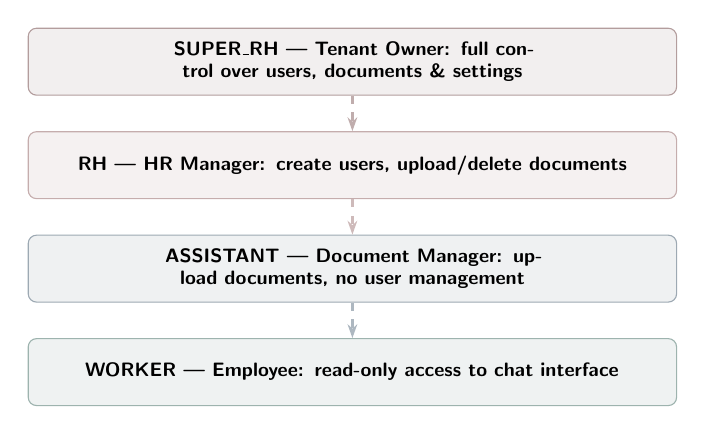
\begin{tikzpicture}[node distance=0.55cm]
  % Four stacked roles, each wider with enough text room
  \node[proc=DeepRose, text width=8cm, minimum height=0.85cm]  (srh)  {\textbf{SUPER\_RH} \textemdash{} Tenant Owner: full control over users, documents \& settings};
  \node[proc=MutedRose, text width=8cm, minimum height=0.85cm, below=0.45cm of srh]  (rh)   {\textbf{RH} \textemdash{} HR Manager: create users, upload/delete documents};
  \node[proc=ABlue,    text width=8cm, minimum height=0.85cm, below=0.45cm of rh]   (asst) {\textbf{ASSISTANT} \textemdash{} Document Manager: upload documents, no user management};
  \node[proc=AMint,    text width=8cm, minimum height=0.85cm, below=0.45cm of asst] (wkr)  {\textbf{WORKER} \textemdash{} Employee: read-only access to chat interface};

  \draw[arr=DeepRose!50, dashed] (srh.south)  -- (rh.north);
  \draw[arr=MutedRose!50,dashed] (rh.south)   -- (asst.north);
  \draw[arr=ABlue!50,   dashed] (asst.south)  -- (wkr.north);
\end{tikzpicture}
\end{center}

\vspace{6pt}

\begin{table}[htbp]
\centering
\caption{Role Permissions Matrix}
\renewcommand{\arraystretch}{1.35}
\begin{tabularx}{\linewidth}{>{\bfseries\sffamily}X c c c c}
\toprule
\rowcolor{DeepRose!12}
Permission & SUPER\_RH & RH & ASSISTANT & WORKER \\
\midrule
Create / Delete Users     & \checkmark & \checkmark & --- & --- \\
Upload Documents          & \checkmark & \checkmark & \checkmark & --- \\
Delete Documents          & \checkmark & \checkmark & --- & --- \\
Preview Documents         & \checkmark & \checkmark & \checkmark & --- \\
Chat with Knowledge Base  & \checkmark & \checkmark & \checkmark & \checkmark \\
Reset User Password       & \checkmark & \checkmark & --- & --- \\
\bottomrule
\end{tabularx}
\end{table}

% ==============================================================
% CHAPTER 2 — HIGH-LEVEL ARCHITECTURE
% ==============================================================
\clearpage
\chapter{High-Level System Architecture}

\section{The Microservices Design Philosophy}

DokuMind deliberately separates concerns across two microservices, each chosen for its optimal fit to the task:

\begin{infobox}
Different computational workloads require different runtimes. JWT validation, transactional database writes, and streaming proxying are best served by the JVM. Dense tensor embedding and neural model inference require Python's AI library ecosystem. Serving static assets requires a lightweight HTTP server like Nginx.
\end{infobox}

\section{Full System Architecture}

\begin{figure}[htbp]
\centering
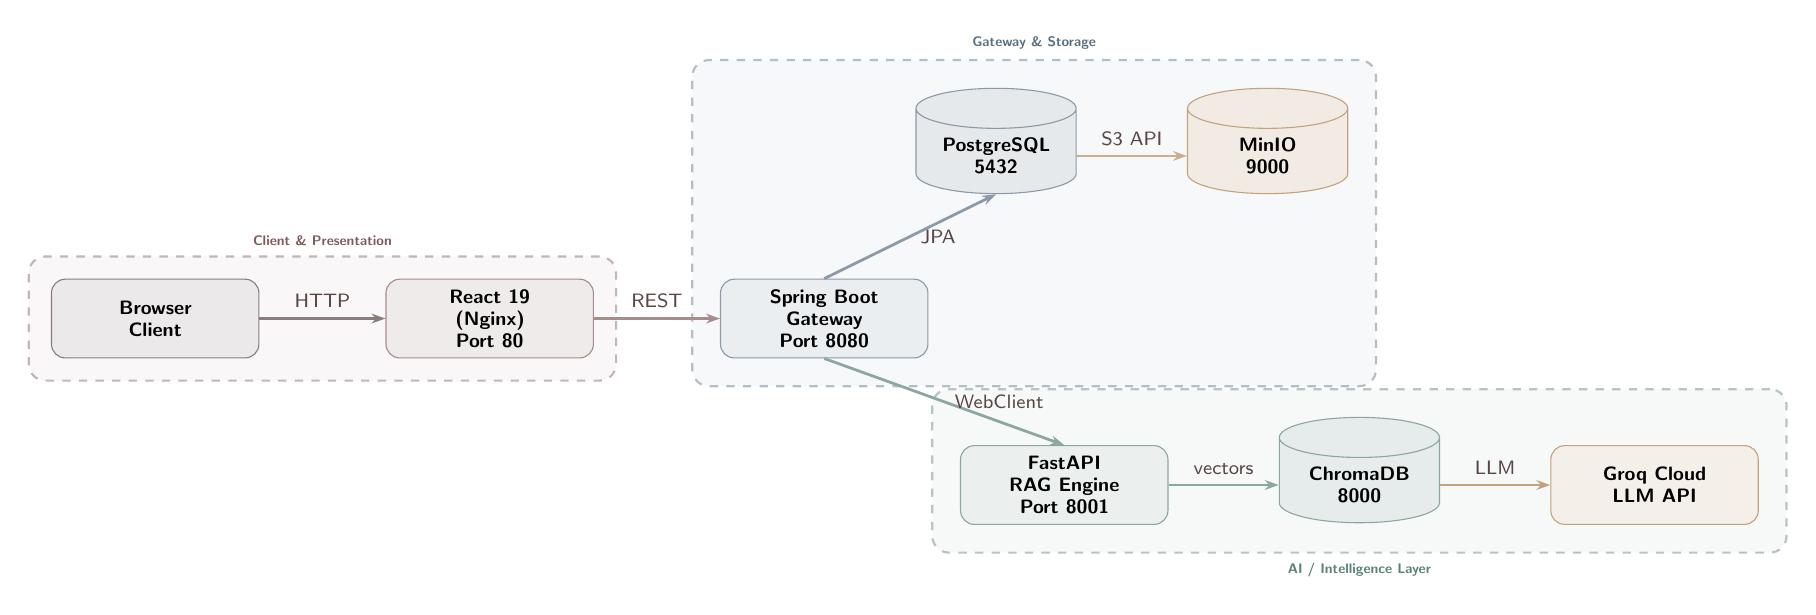
\begin{tikzpicture}[node distance=0.8cm and 1.6cm]

  % ---- ROW 1: Client  →  Frontend  →  Gateway ----
  \node[svc=DarkEarth] (user) {Browser\\Client};
  \node[svc=DeepRose,  right=1.6cm of user] (fe) {React 19\\(Nginx)\\Port 80};
  \node[svc=ABlue,     right=1.6cm of fe]   (gw) {Spring Boot\\Gateway\\Port 8080};

  % ---- ROW 2 (above gateway): data stores ----
  \node[dbs=ABlue,   above right=1.1cm and 0.4cm of gw] (pg)    {PostgreSQL\\5432};
  \node[dbs=AAmber,  right=1.4cm of pg]                 (minio) {MinIO\\9000};

  % ---- ROW 3 (below gateway): AI layer ----
  \node[svc=AMint,   below right=1.1cm and 0.4cm of gw] (rag)   {FastAPI\\RAG Engine\\Port 8001};
  \node[dbs=AMint,   right=1.4cm of rag]                (chroma){ChromaDB\\8000};
  \node[svc=AAmber,  right=1.4cm of chroma]             (groq)  {Groq Cloud\\LLM API};

  % ---- ARROWS ----
  \draw[arr=DarkEarth!70] (user) -- node[above,lbl]{HTTP}      (fe);
  \draw[arr=DeepRose!70]  (fe)   -- node[above,lbl]{REST}       (gw);
  \draw[arr=ABlue!70]     (gw.north) -- node[right,lbl]{JPA}   (pg.south);
  \draw[arr=AAmber!60]    (pg.east)  -- node[above,lbl]{S3 API}(minio.west);
  \draw[arr=AMint!70]     (gw.south) -- node[right,lbl]{WebClient} (rag.north);
  \draw[arr=AMint!70]     (rag.east) -- node[above,lbl]{vectors}   (chroma.west);
  \draw[arr=AAmber!70]    (chroma.east)--node[above,lbl]{LLM}      (groq.west);

  % ---- GROUP BOXES ----
  \begin{scope}[on background layer]
    \node[grp=DeepRose, fit=(user)(fe), inner sep=8pt,
      label={[font=\sffamily\tiny\bfseries\color{DeepRose}]above:Client \& Presentation}] {};
    \node[grp=ABlue, fit=(gw)(pg)(minio), inner sep=10pt,
      label={[font=\sffamily\tiny\bfseries\color{ABlue}]above:Gateway \& Storage}] {};
    \node[grp=AMint, fit=(rag)(chroma)(groq), inner sep=10pt,
      label={[font=\sffamily\tiny\bfseries\color{AMint}]below:AI / Intelligence Layer}] {};
  \end{scope}

\end{tikzpicture}
\caption{Full DokuMind system topology: services, databases, and data flows.}
\label{fig:arch_full}
\end{figure}

\section{End-to-End Workflow}

\subsection{Document Ingestion Workflow}
\begin{enumerate}[label=\arabic*.]
  \item User uploads a PDF via the React frontend (\texttt{POST /documents/ingest}).
  \item The \texttt{JwtFilter} validates the Bearer token and extracts the \texttt{companyId}.
  \item \texttt{DocumentService} stores the raw PDF in MinIO under the key \texttt{companyId/filename.pdf}.
  \item Simultaneously, the Gateway forwards the PDF bytes + \texttt{tenantId} to the FastAPI RAG service via a non-blocking \texttt{WebClient} request.
  \item The RAG service parses, chunks, embeds, and indexes the text into a tenant-specific ChromaDB collection.
  \item The Gateway returns HTTP~200 to the frontend.
\end{enumerate}

\subsection{Grounded Chat Workflow}
\begin{enumerate}[label=\arabic*.]
  \item The user submits a question via the chat UI.
  \item The Gateway proxies the request (with \texttt{tenantId}) to the FastAPI \texttt{/api/chat} endpoint.
  \item The RAG pipeline retrieves, reranks, and gates the context chunks.
  \item If context passes the similarity threshold, the pipeline calls the Groq LLM API.
  \item The response is streamed back through Spring WebFlux as a Server-Sent Event (SSE).
  \item The React frontend renders tokens incrementally, creating a live typing effect.
\end{enumerate}

\section{Technology Stack}

\begin{table}[htbp]
\centering
\caption{DokuMind Complete Technology Stack}
\renewcommand{\arraystretch}{1.35}
\begin{tabularx}{\linewidth}{>{\bfseries\sffamily\color{DeepRose}}l >{\ttfamily}l X}
\toprule
\rowcolor{DeepRose!10}
Layer & Version & Role \\
\midrule
React             & 19.2.6        & SPA UI framework \\
Vite              & 8.0.12        & Build tool and HMR dev server \\
TypeScript        & \texttildelow6.0 & Static type safety \\
Tailwind CSS      & 4.3.0         & Utility-first styling engine \\
Framer Motion     & 12.40.0       & UI animations \\
Axios             & 1.16.1        & HTTP client with JWT interceptors \\
Radix UI / Shadcn & \textasciicircum1.4.3 & Accessible UI primitives \\
\midrule
Spring Boot       & 4.0.5         & Orchestration gateway and REST API \\
Java              & 21 (Temurin)  & JVM runtime \\
Spring Security   & Boot default  & JWT auth, CORS, RBAC enforcement \\
Spring WebFlux    & Boot default  & Reactive streaming via WebClient \\
Spring Data JPA   & Boot default  & ORM and transactional repositories \\
Spring Mail       & 4.0.5         & SMTP email for user provisioning \\
JJWT              & 0.13.0        & JWT signing and validation \\
MinIO SDK         & 8.5.10        & S3-compatible object storage client \\
Lombok            & 1.18.x        & Compile-time boilerplate generation \\
\midrule
FastAPI           & 0.135.3       & Async HTTP router and validator \\
Python            & 3.11-slim     & AI library runtime \\
Uvicorn           & 0.43.0        & ASGI production server \\
LangChain Classic & 1.0.3         & Parent-Document retriever \\
sentence-transformers & 5.3.0     & Dense embedding + Cross-Encoder reranker \\
pypdf             & 6.9.2         & PDF text extraction \\
groq (SDK)        & < 1.0.0       & Groq Cloud LLM API client \\
Pydantic Settings & latest        & Config management via environment vars \\
\midrule
PostgreSQL        & 15            & Relational DB: users, tokens, companies \\
MinIO             & latest        & S3-compatible PDF object store \\
ChromaDB          & latest        & Distributed vector database server \\
Docker Compose    & v2            & Container orchestration \\
Nginx             & alpine        & Static frontend serving \\
\bottomrule
\end{tabularx}
\end{table}

% ==============================================================
% CHAPTER 3 — PLATFORM GATEWAY
% ==============================================================
\clearpage
\chapter{Platform Gateway --- Spring Boot Orchestrator}

\section{Overview of Responsibilities}

The Platform Gateway is the single point of entry for all client requests:

\begin{center}
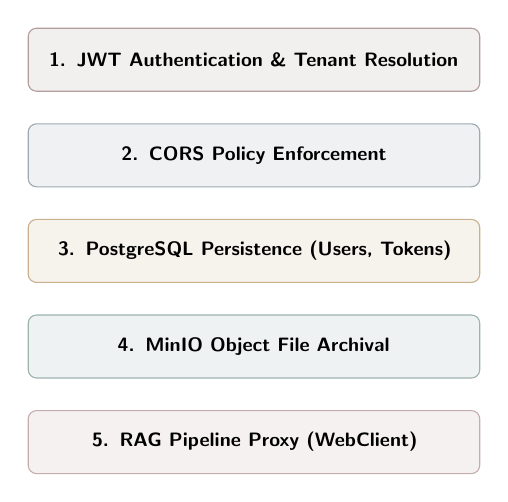
\begin{tikzpicture}[node distance=0.5cm]
  \node[proc=DeepRose,  text width=5.5cm, minimum height=0.8cm] (a) {1. JWT Authentication \& Tenant Resolution};
  \node[proc=ABlue,     text width=5.5cm, minimum height=0.8cm, below=0.4cm of a] (b) {2. CORS Policy Enforcement};
  \node[proc=AAmber,    text width=5.5cm, minimum height=0.8cm, below=0.4cm of b] (c) {3. PostgreSQL Persistence (Users, Tokens)};
  \node[proc=AMint,     text width=5.5cm, minimum height=0.8cm, below=0.4cm of c] (d) {4. MinIO Object File Archival};
  \node[proc=MutedRose, text width=5.5cm, minimum height=0.8cm, below=0.4cm of d] (e) {5. RAG Pipeline Proxy (WebClient)};
\end{tikzpicture}
\end{center}

\section{Security Architecture \& JWT Flow}

\subsection{The JwtFilter Mechanism}

Every HTTP request passing through the Gateway is intercepted by the custom \texttt{JwtFilter} (an implementation of Spring's \texttt{OncePerRequestFilter}).

\begin{figure}[htbp]
\centering
% Vertical layout avoids horizontal overflow
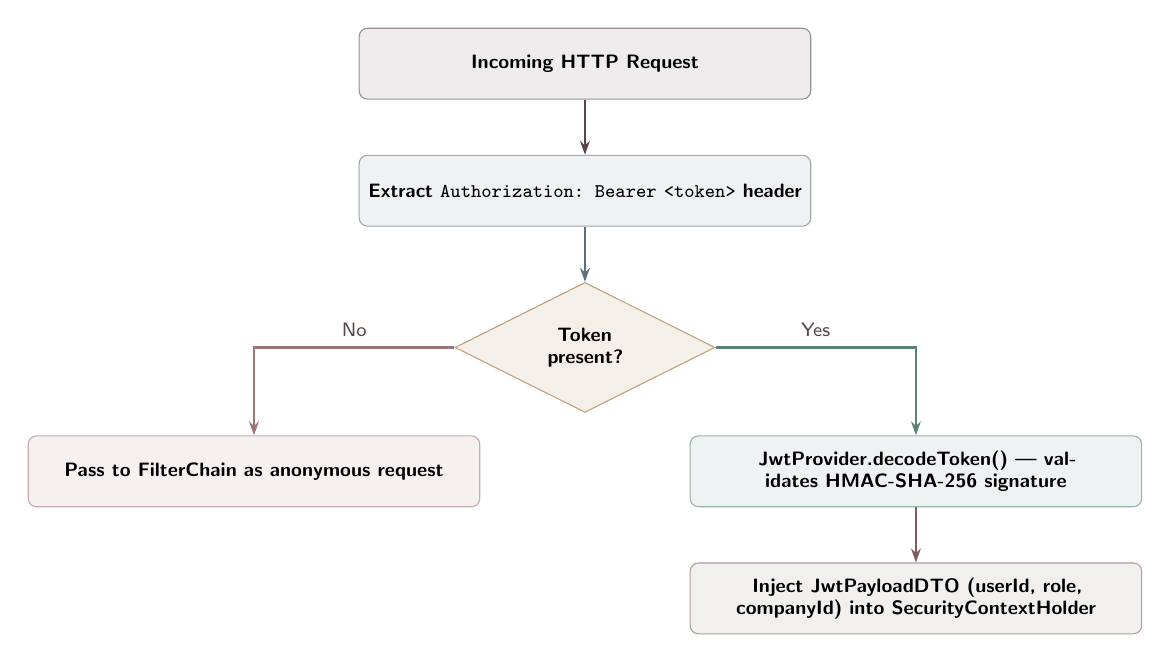
\begin{tikzpicture}[node distance=0.7cm]
  \node[proc=DarkEarth, text width=5.5cm] (req)     {Incoming HTTP Request};
  \node[proc=ABlue,     text width=5.5cm, below=0.7cm of req]    (extract) {Extract \texttt{Authorization: Bearer <token>} header};
  \node[dec,                              below=0.7cm of extract] (hastoken){Token\\present?};
  \node[proc=AMint,     text width=5.5cm, below right=0.7cm and 0.5cm of hastoken] (decode)  {JwtProvider.decodeToken() — validates HMAC-SHA-256 signature};
  \node[proc=DeepRose,  text width=5.5cm, below=0.7cm of decode]  (inject)  {Inject JwtPayloadDTO (userId, role, companyId) into SecurityContextHolder};
  \node[proc=MutedRose, text width=5.5cm, below left=0.7cm and 0.5cm of hastoken]  (chain)   {Pass to FilterChain as anonymous request};

  \draw[arr=DarkEarth] (req)     -- (extract);
  \draw[arr=ABlue]     (extract) -- (hastoken);
  \draw[arr=AMint]     (hastoken.east) -| node[near start,above,lbl]{Yes} (decode.north);
  \draw[arr=DeepRose]  (decode)  -- (inject);
  \draw[arr=MutedRose] (hastoken.west) -| node[near start,above,lbl]{No}  (chain.north);
\end{tikzpicture}
\caption{JwtFilter: step-by-step execution flow for every incoming API request.}
\label{fig:jwt_filter}
\end{figure}

The \texttt{JwtProvider.decodeToken()} method extracts three critical claims from the JWT payload:

\begin{itemize}
  \item \textbf{subject} — the User UUID (e.g., \texttt{550e8400-e29b-41d4-a716-446655440000})
  \item \textbf{role} — one of \texttt{SUPER\_RH | RH | ASSISTANT | WORKER}
  \item \textbf{companyId} — the tenant UUID used for all data isolation
\end{itemize}

These are packaged into a \texttt{JwtPayloadDTO} record and injected into the \texttt{SecurityContextHolder}, making them instantly available to any service method without additional database queries.

\subsection{Dual-Token Security Model}

\begin{figure}[htbp]
\centering
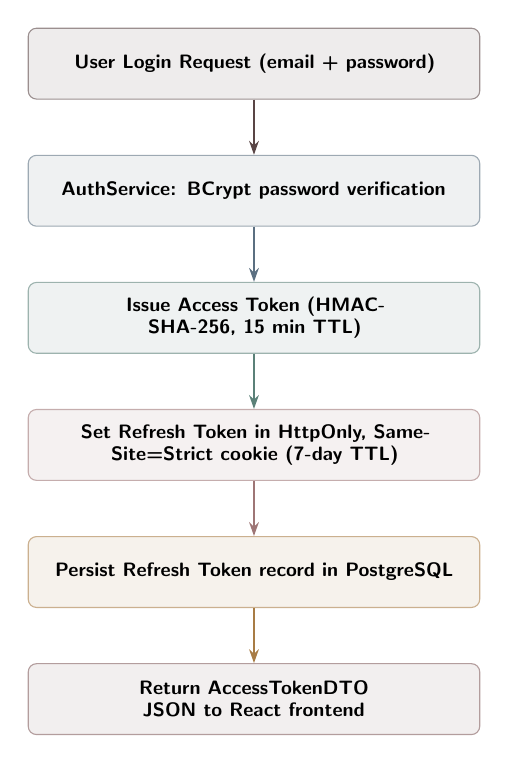
\begin{tikzpicture}[node distance=0.7cm]
  \node[proc=DarkEarth, text width=5.5cm] (login)  {User Login Request (email + password)};
  \node[proc=ABlue,     text width=5.5cm, below=0.7cm of login]  (verify) {AuthService: BCrypt password verification};
  \node[proc=AMint,     text width=5.5cm, below=0.7cm of verify] (issue)  {Issue Access Token (HMAC-SHA-256, 15 min TTL)};
  \node[proc=MutedRose, text width=5.5cm, below=0.7cm of issue]  (cookie) {Set Refresh Token in HttpOnly, SameSite=Strict cookie (7-day TTL)};
  \node[proc=AAmber,    text width=5.5cm, below=0.7cm of cookie] (store)  {Persist Refresh Token record in PostgreSQL};
  \node[proc=DeepRose,  text width=5.5cm, below=0.7cm of store]  (resp)   {Return AccessTokenDTO JSON to React frontend};

  \draw[arr=DarkEarth] (login)  -- (verify);
  \draw[arr=ABlue]     (verify) -- (issue);
  \draw[arr=AMint]     (issue)  -- (cookie);
  \draw[arr=MutedRose] (cookie) -- (store);
  \draw[arr=AAmber]    (store)  -- (resp);
\end{tikzpicture}
\caption{Dual-token authentication issuance lifecycle.}
\label{fig:dual_token}
\end{figure}

\begin{warningbox}
\textbf{Security Design:} The Refresh Token is stored in an \texttt{HttpOnly} cookie — completely inaccessible to JavaScript — preventing XSS attacks. Access Tokens live only in React's memory (never in \texttt{localStorage}). Both tokens are signed with \emph{separate} HMAC secrets, so a stolen Access Token cannot forge a Refresh Token.
\end{warningbox}

\subsection{Silent Token Refresh}

When the Access Token expires, the Axios interceptor in \texttt{AuthProvider.tsx} transparently:
\begin{enumerate}[label=\arabic*.]
  \item Catches the \texttt{401 Unauthorized} before it reaches any UI component.
  \item Suspends all pending API requests in a queue.
  \item Issues a silent \texttt{GET /auth/refresh}; the browser automatically sends the \texttt{HttpOnly} cookie.
  \item Spring Boot validates and issues a new Access Token.
  \item The interceptor replays all queued requests — the user sees zero disruption.
\end{enumerate}

\section{Domain Model \& Relational Schema}

\subsection{Entity Relationship Diagram}

\begin{figure}[htbp]
\centering
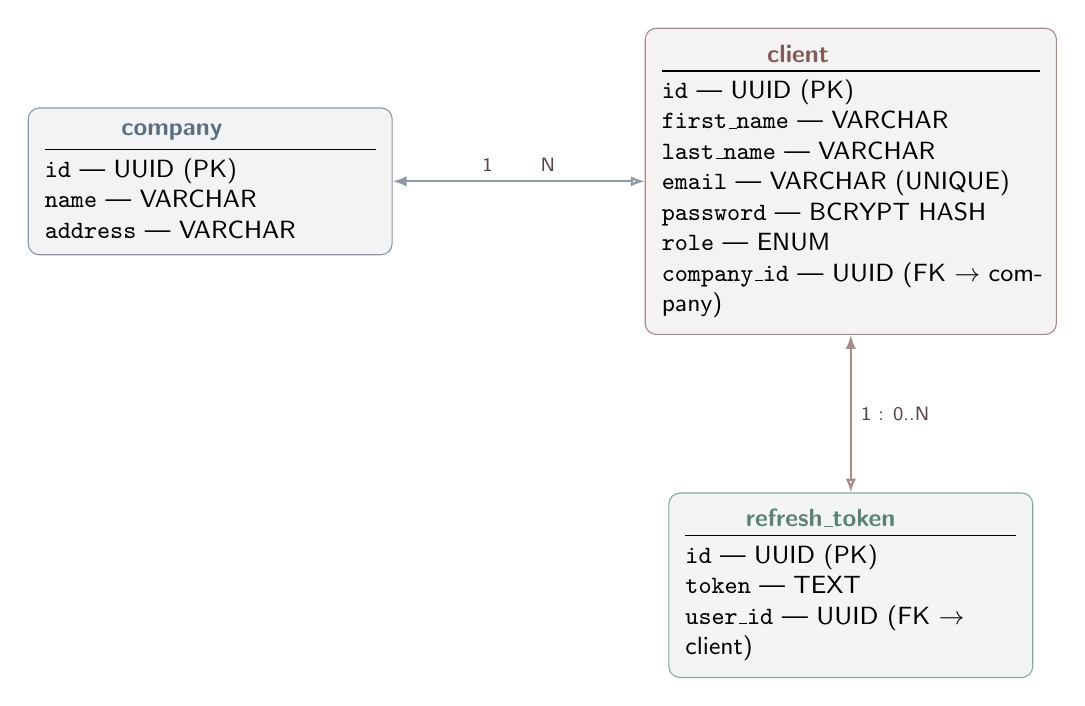
\begin{tikzpicture}[node distance=2.5cm, every node/.style={font=\sffamily\small}]

  % Company
  \node[draw=ABlue!70, fill=ABlue!8, rounded corners=4pt,
        text width=4.2cm, align=left, inner sep=6pt] (company) {
    \textbf{\color{ABlue}\hfil company\hfil}\\[3pt]
    \hrule\vspace{3pt}
    \texttt{id} \textemdash{} UUID (PK)\\
    \texttt{name} \textemdash{} VARCHAR\\
    \texttt{address} \textemdash{} VARCHAR
  };

  % User/client
  \node[draw=DeepRose!70, fill=DeepRose!8, rounded corners=4pt,
        text width=4.8cm, align=left, inner sep=6pt, right=3.2cm of company] (usr) {
    \textbf{\color{DeepRose}\hfil client\hfil}\\[3pt]
    \hrule\vspace{3pt}
    \texttt{id} \textemdash{} UUID (PK)\\
    \texttt{first\_name} \textemdash{} VARCHAR\\
    \texttt{last\_name} \textemdash{} VARCHAR\\
    \texttt{email} \textemdash{} VARCHAR (UNIQUE)\\
    \texttt{password} \textemdash{} BCRYPT HASH\\
    \texttt{role} \textemdash{} ENUM\\
    \texttt{company\_id} \textemdash{} UUID (FK $\to$ company)
  };

  % RefreshToken
  \node[draw=AMint!70, fill=AMint!8, rounded corners=4pt,
        text width=4.2cm, align=left, inner sep=6pt, below=2cm of usr] (rt) {
    \textbf{\color{AMint}\hfil refresh\_token\hfil}\\[3pt]
    \hrule\vspace{3pt}
    \texttt{id} \textemdash{} UUID (PK)\\
    \texttt{token} \textemdash{} TEXT\\
    \texttt{user\_id} \textemdash{} UUID (FK $\to$ client)
  };

  % Relations
  \draw[{Latex[length=5pt]}-{Latex[length=5pt,open]}, thick, color=ABlue!70]
    (company.east) -- node[above,font=\sffamily\scriptsize,color=DarkEarth]{1 \quad\quad N}(usr.west);
  \draw[{Latex[length=5pt]}-{Latex[length=5pt,open]}, thick, color=DeepRose!70]
    (usr.south) -- node[right,font=\sffamily\scriptsize,color=DarkEarth]{1 : 0..N} (rt.north);

\end{tikzpicture}
\caption{PostgreSQL Entity Relationship Diagram showing the tenant isolation model.}
\label{fig:erd}
\end{figure}

\subsection{The Company--User Relationship}
Every \texttt{User} entity carries a non-nullable FK to a \texttt{Company}. All repository queries are filtered by the authenticated user's \texttt{companyId}, so Company A's data is never returned to Company B's users.

\section{MinIO Object Storage Integration}

\begin{figure}[htbp]
\centering
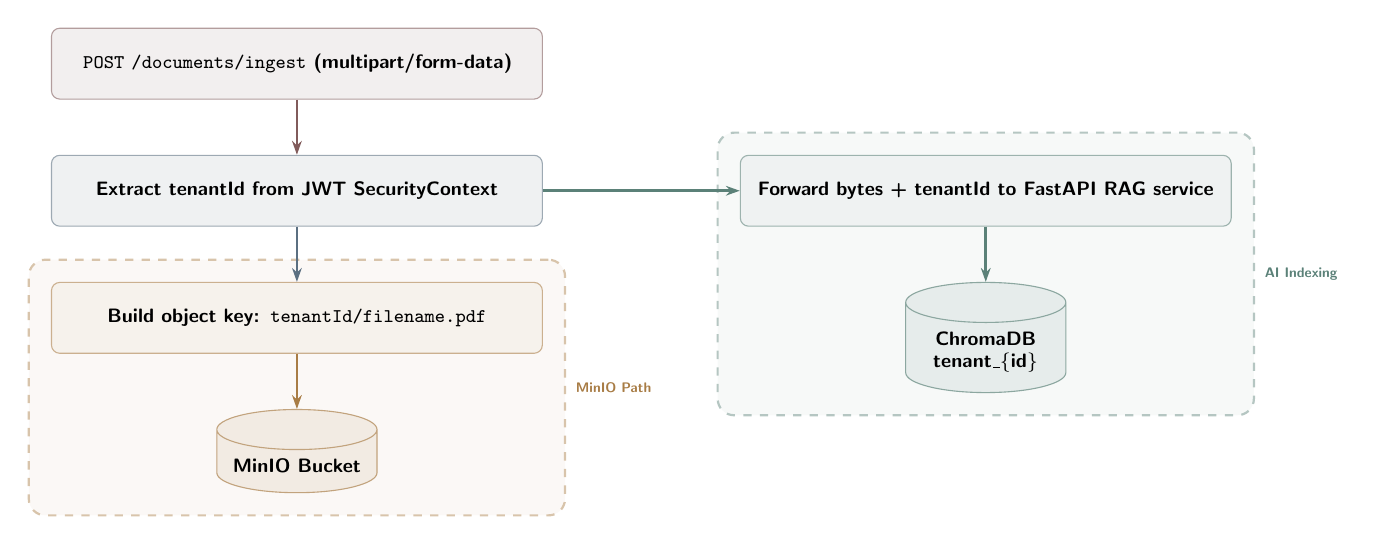
\begin{tikzpicture}[node distance=0.7cm]
  % Vertical flow — guaranteed no overlap
  \node[proc=DeepRose, text width=6cm] (upload) {\texttt{POST /documents/ingest} (multipart/form-data)};
  \node[proc=ABlue,    text width=6cm, below=0.7cm of upload] (extract){Extract tenantId from JWT SecurityContext};
  \node[proc=AAmber,   text width=6cm, below=0.7cm of extract](key)    {Build object key: \texttt{tenantId/filename.pdf}};
  \node[dbs=AAmber,    below=0.7cm of key]  (minio) {MinIO Bucket};

  \node[proc=AMint,    text width=6cm, right=2.5cm of extract](rag) {Forward bytes + tenantId to FastAPI RAG service};
  \node[dbs=AMint,     below=0.7cm of rag]  (chroma){ChromaDB\\tenant\_\{id\}};

  \draw[arr=DeepRose] (upload)  -- (extract);
  \draw[arr=ABlue]    (extract) -- (key);
  \draw[arr=AAmber]   (key)     -- (minio);
  \draw[arr=AMint]    (extract.east) -- (rag.west);
  \draw[arr=AMint]    (rag)     -- (chroma);

  \begin{scope}[on background layer]
    \node[grp=AAmber, fit=(key)(minio), inner sep=8pt,
      label={[font=\sffamily\tiny\bfseries\color{AAmber}]right:MinIO Path}] {};
    \node[grp=AMint, fit=(rag)(chroma), inner sep=8pt,
      label={[font=\sffamily\tiny\bfseries\color{AMint}]right:AI Indexing}] {};
  \end{scope}

\end{tikzpicture}
\caption{Document ingestion: MinIO archival and RAG vectorisation run concurrently.}
\label{fig:ingest_flow}
\end{figure}

\section{Reactive Streaming with WebClient}

The \texttt{RagPipelineService} uses Spring WebFlux's \texttt{WebClient} — a non-blocking HTTP client. While Python streams tokens from Groq, the Spring thread is released to serve other requests. As each token arrives, it is immediately forwarded as a Server-Sent Event (SSE) to the browser, creating the real-time typing animation.

\section{User Lifecycle \& Email Provisioning}

When an administrator creates a new user, \texttt{UserService.createUser()} executes the following transaction:

\begin{enumerate}[label=\arabic*.]
  \item Validates the admin's \texttt{companyId} exists in PostgreSQL.
  \item Enforces RBAC constraints (e.g., an \texttt{RH} cannot create another \texttt{RH}).
  \item Generates a cryptographically random temporary password via \texttt{BcryptUtility.generateRandomPassword()}.
  \item Hashes it using BCrypt and saves the \texttt{User} entity bound to the \texttt{companyId}.
  \item Dispatches an HTML welcome email via \texttt{JavaMailSender} containing the user's initial credentials.
\end{enumerate}

% ==============================================================
% CHAPTER 4 — FRONTEND
% ==============================================================
\clearpage
\chapter{Frontend Client Application}

\section{SPA Architecture \& Component Structure}

The presentation layer is built with React~19, bundled by Vite~8, and written entirely in TypeScript.

\begin{techbox}{Project Directory Structure}
\begin{lstlisting}[numbers=none, frame=none, backgroundcolor=\color{CodeBg}]
FrontEnd/src/
  App.tsx             -- Root router: role-based page mapping
  main.tsx            -- ReactDOM.createRoot, wraps <AuthProvider>
  context/
    AuthProvider.tsx  -- JWT lifecycle, Axios interceptors
  services/
    apiClient.ts      -- Axios instances (withCredentials=true)
  hooks/
    useDocuments.ts   -- PDF upload, preview, delete state
  pages/
    auth/             -- Login and Sign-Up pages
    admin/            -- SUPER_RH: full CRUD dashboard
    rh/               -- RH: user + document management
    assistant/        -- ASSISTANT: document management only
    worker/           -- WORKER: chat interface only
    chat/             -- SSE streaming chat workspace
  components/         -- Shared Navbar, Sidebar, modals
  types/              -- TypeScript API payload interfaces
\end{lstlisting}
\end{techbox}

\section{Authentication Context \& Axios Interceptors}

\begin{figure}[htbp]
\centering
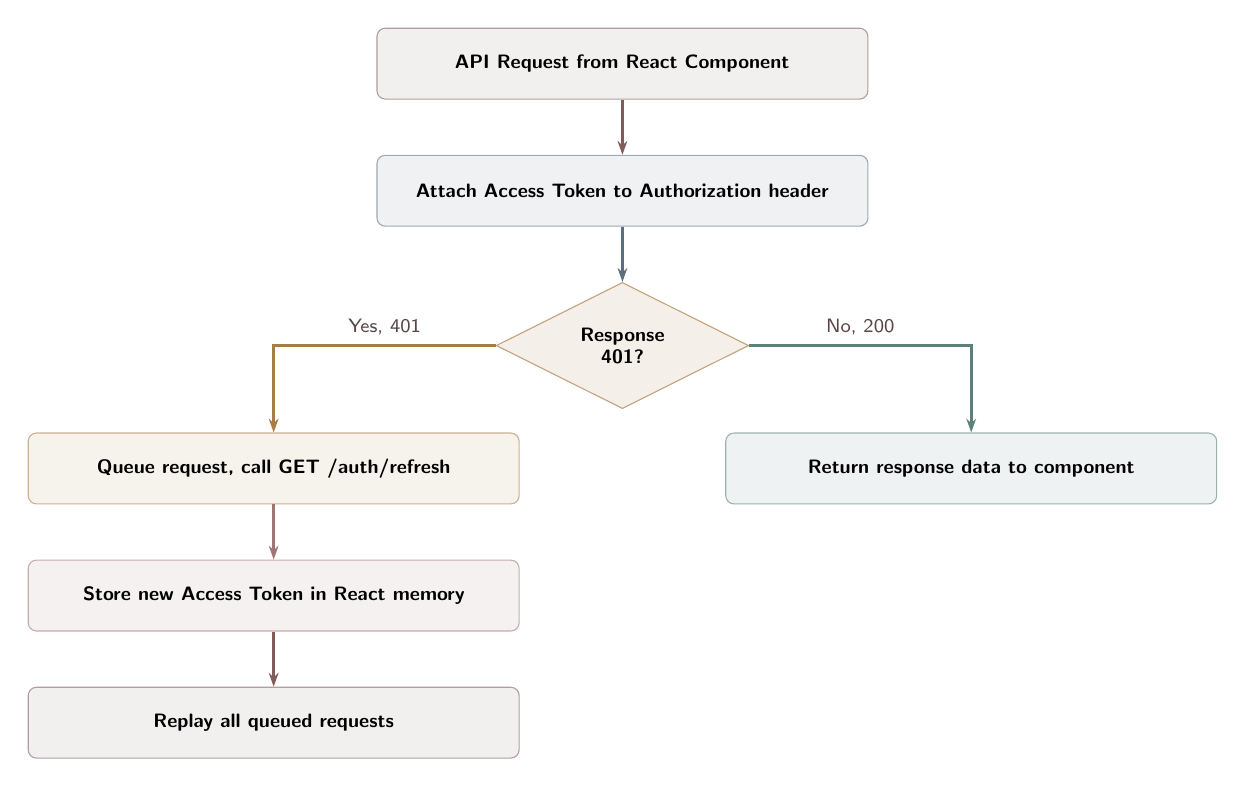
\begin{tikzpicture}[node distance=0.7cm]
  \node[proc=DeepRose, text width=6cm] (request) {API Request from React Component};
  \node[proc=ABlue,    text width=6cm, below=0.7cm of request]  (attach)  {Attach Access Token to Authorization header};
  \node[dec,                           below=0.7cm of attach]   (resp)    {Response\\401?};
  \node[proc=AMint,    text width=6cm, below right=0.7cm and 0.5cm of resp] (ok)      {Return response data to component};
  \node[proc=AAmber,   text width=6cm, below left=0.7cm and 0.5cm of resp]  (queue)   {Queue request, call GET /auth/refresh};
  \node[proc=MutedRose,text width=6cm, below=0.7cm of queue]   (newtoken){Store new Access Token in React memory};
  \node[proc=DeepRose, text width=6cm, below=0.7cm of newtoken] (replay)  {Replay all queued requests};

  \draw[arr=DeepRose] (request)  -- (attach);
  \draw[arr=ABlue]    (attach)   -- (resp);
  \draw[arr=AMint]    (resp.east) -| node[near start,above,lbl]{No, 200}  (ok.north);
  \draw[arr=AAmber]   (resp.west) -| node[near start,above,lbl]{Yes, 401} (queue.north);
  \draw[arr=MutedRose](queue)    -- (newtoken);
  \draw[arr=DeepRose] (newtoken) -- (replay);
\end{tikzpicture}
\caption{Axios interceptor silent JWT refresh flow — the user experiences zero disruption.}
\label{fig:axios_interceptor}
\end{figure}

\section{UI Walkthrough}

\subsection{Authentication Portals}

\begin{figure}[htbp]
    \centering
    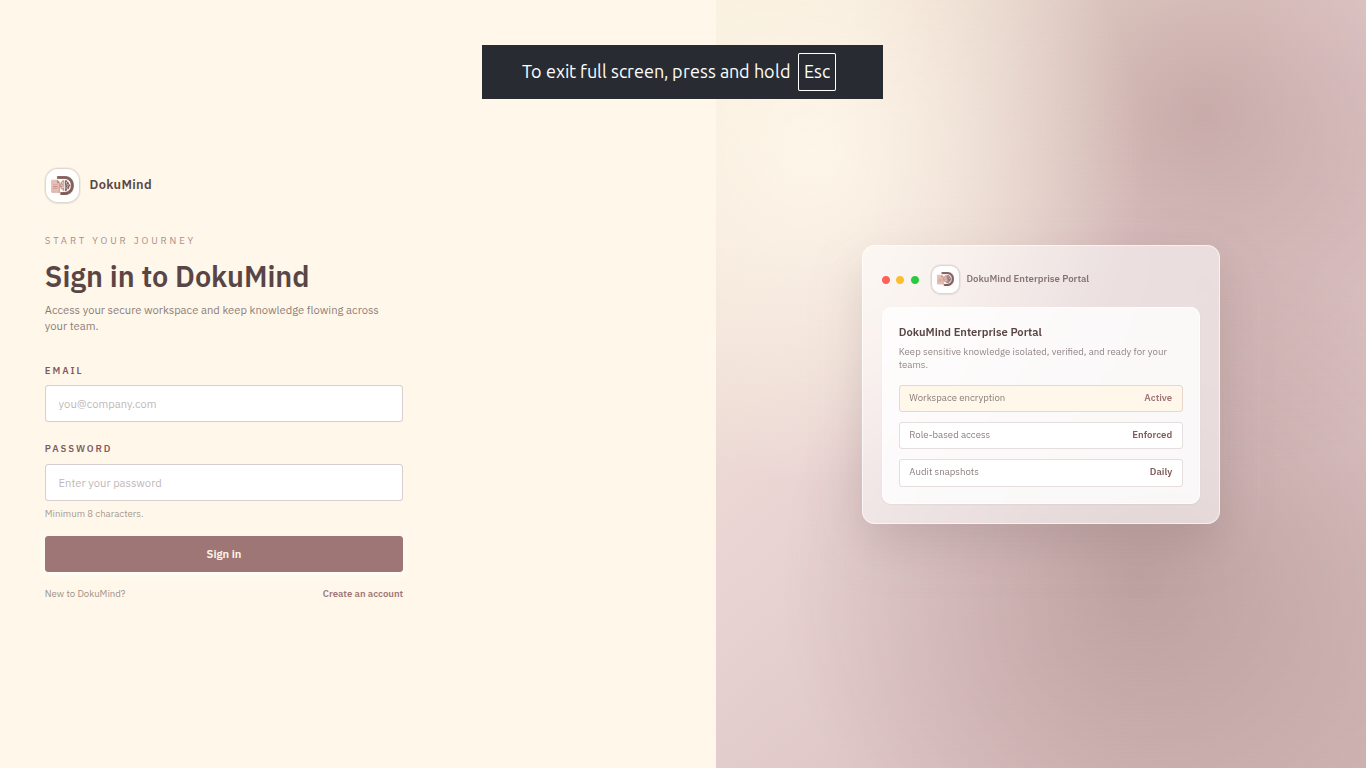
\includegraphics[width=0.9\textwidth]{sign_in_page.png}
    \caption{Login portal with DokuMind brand palette, routing users to their role-specific dashboard.}
    \label{fig:ui_signin}
\end{figure}

\begin{figure}[htbp]
    \centering
    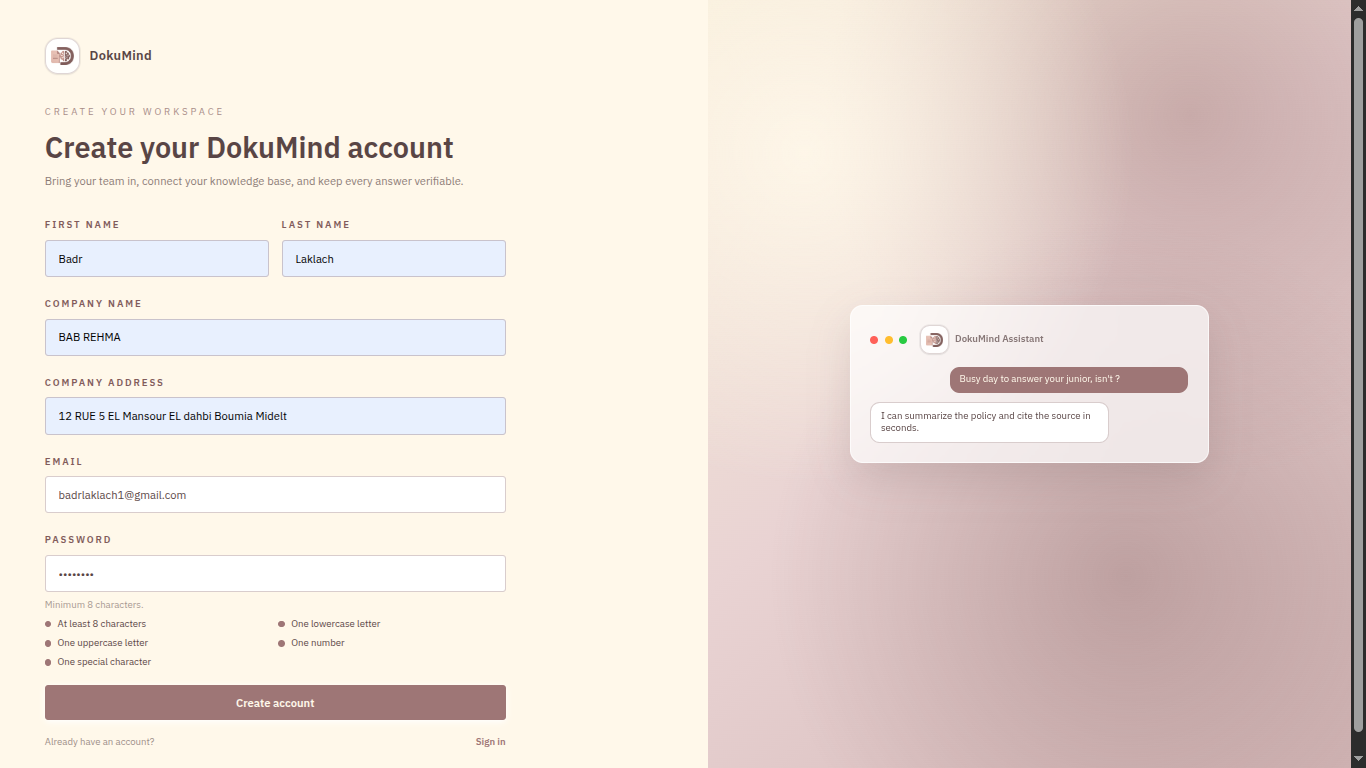
\includegraphics[width=0.9\textwidth]{sign_up_page.png}
    \caption{Tenant onboarding form: creates a Company record and assigns the SUPER\_RH role.}
    \label{fig:ui_signup}
\end{figure}

\clearpage
\subsection{User Management Dashboard}

\begin{figure}[htbp]
    \centering
    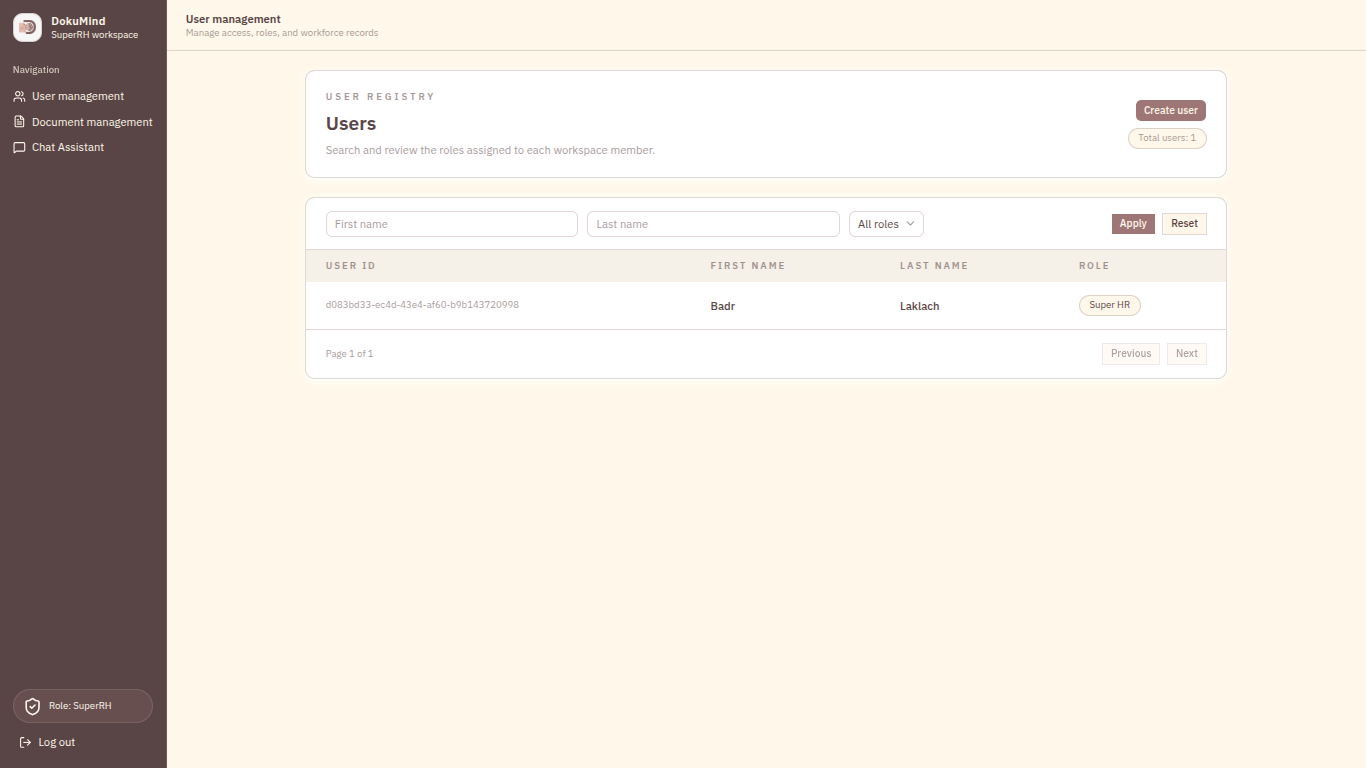
\includegraphics[width=0.9\textwidth]{user_management_page.png}
    \caption{User Management portal: paginated employee directory scoped by the JWT companyId.}
    \label{fig:ui_users}
\end{figure}

\begin{figure}[htbp]
    \centering
    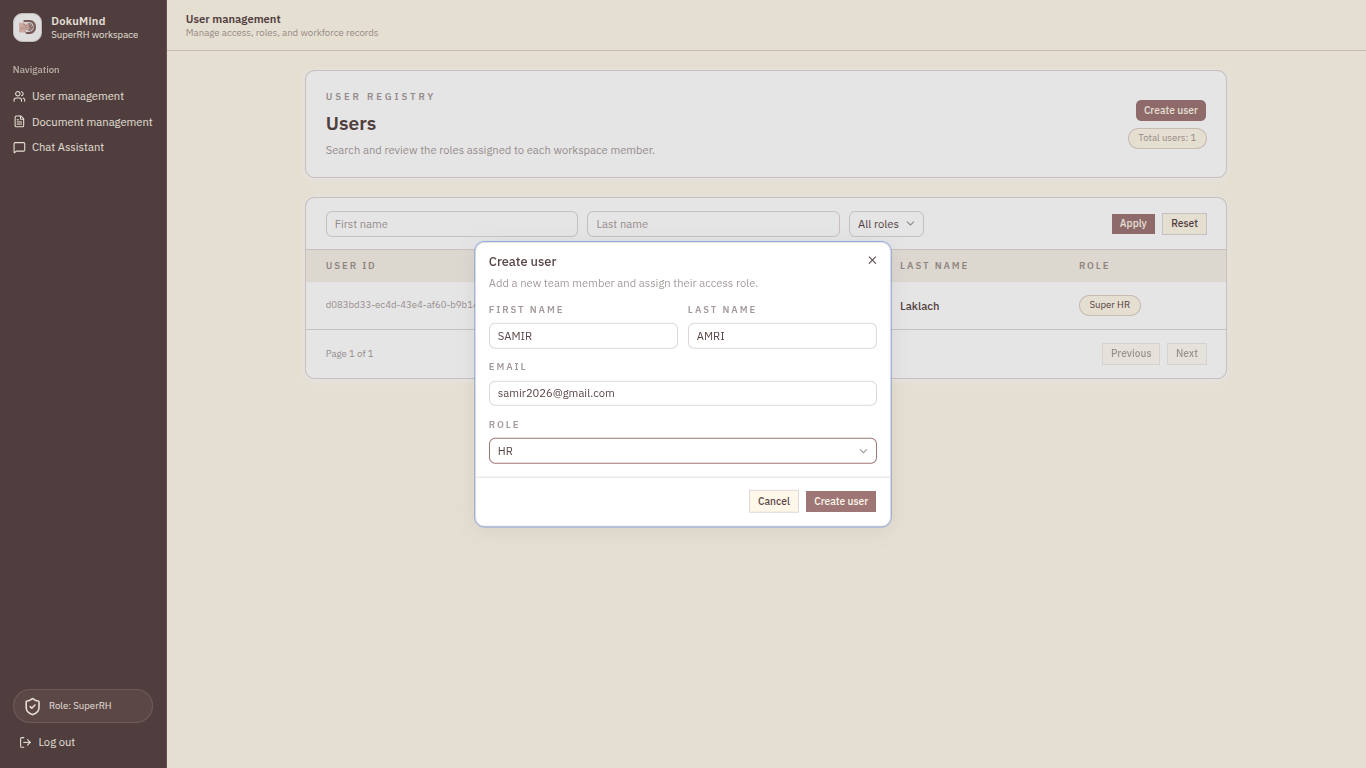
\includegraphics[width=0.9\textwidth]{creating_a_user.png}
    \caption{Create User modal with RBAC role assignment. The server emails credentials on save.}
    \label{fig:ui_createuser}
\end{figure}

\begin{figure}[htbp]
    \centering
    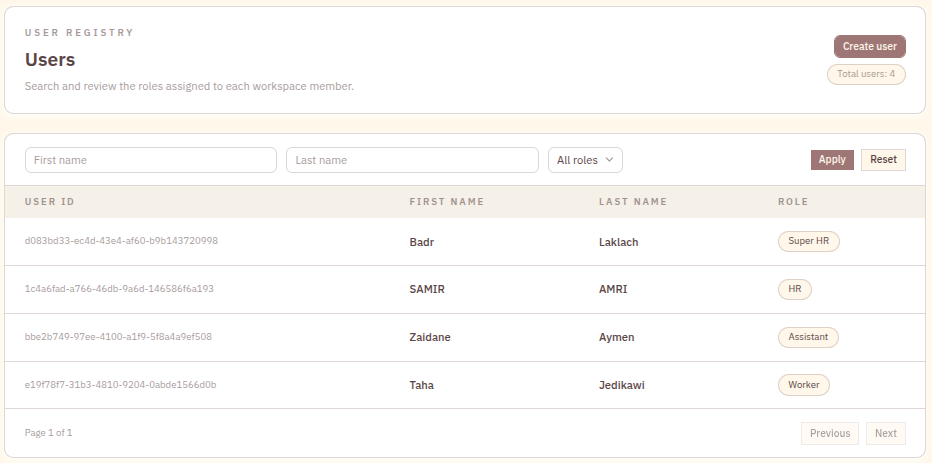
\includegraphics[width=0.9\textwidth]{user_list_after_creation.png}
    \caption{Employee roster after provisioning a new Worker account.}
    \label{fig:ui_userlist}
\end{figure}

\clearpage
\subsection{Document Management Panel}

\begin{figure}[htbp]
    \centering
    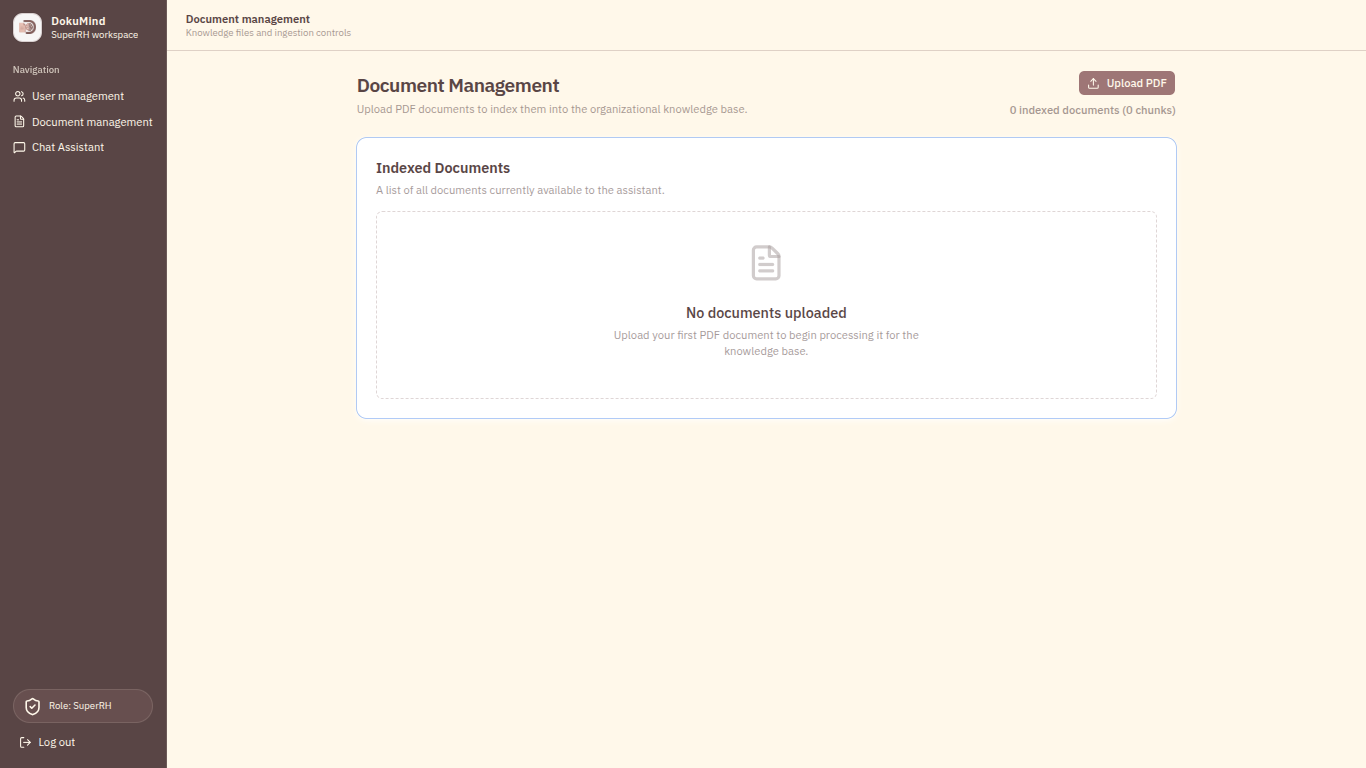
\includegraphics[width=0.9\textwidth]{document_management_page.png}
    \caption{Document Ingestion panel: indexed files shown with their chunk counts.}
    \label{fig:ui_docs}
\end{figure}

\subsection{AI Chat Interface}

\begin{figure}[htbp]
    \centering
    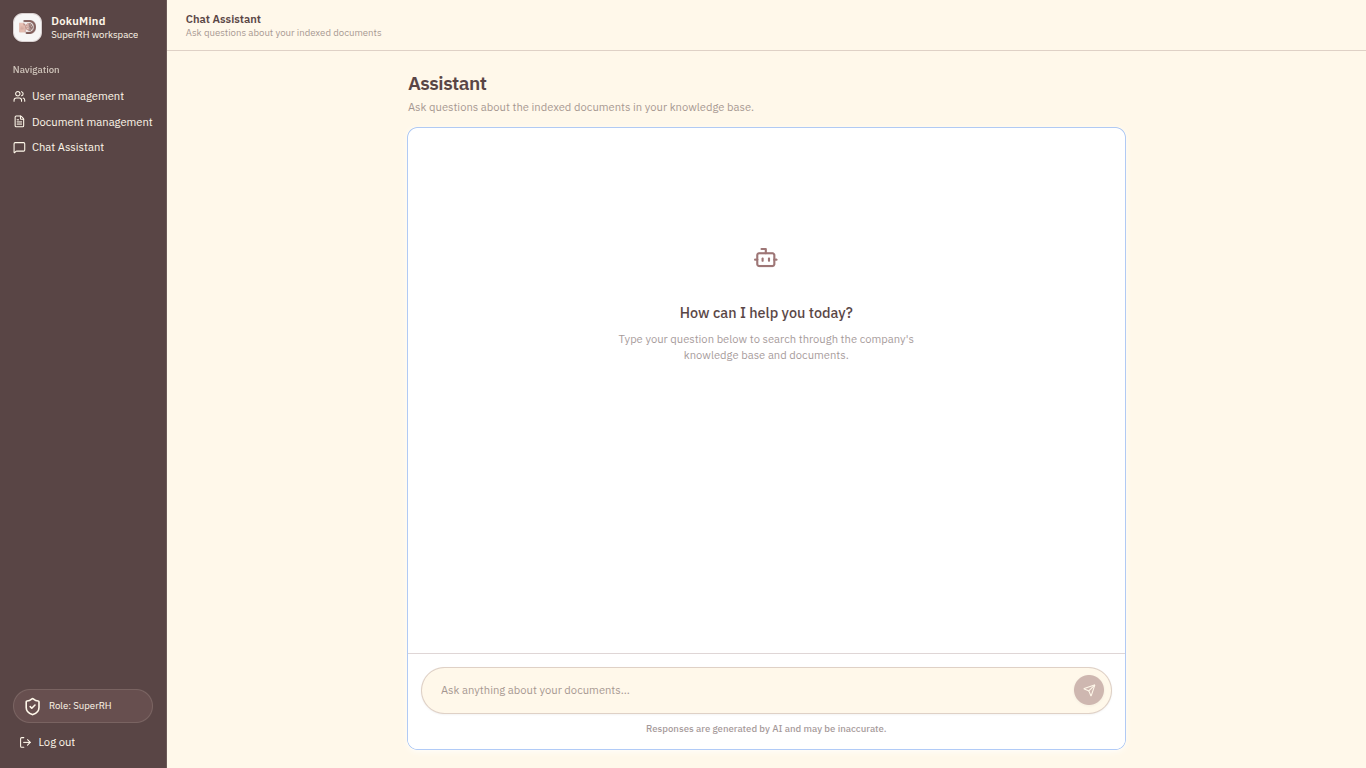
\includegraphics[width=0.9\textwidth]{chat_assistant_page.png}
    \caption{Grounded chat workspace: clean interface awaiting the first employee query.}
    \label{fig:ui_chatempty}
\end{figure}

\begin{figure}[htbp]
    \centering
    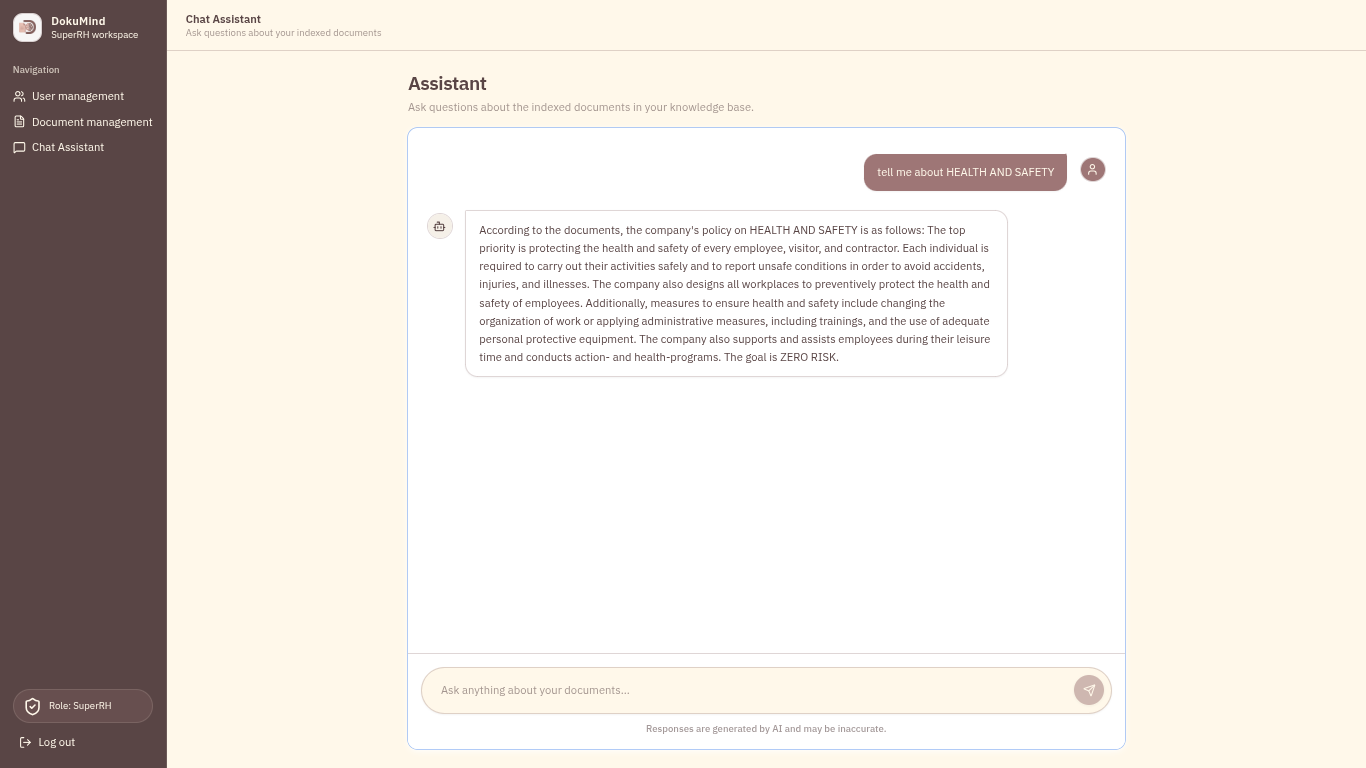
\includegraphics[width=0.9\textwidth]{chatting-example-page_message.png}
    \caption{Live conversational stream with inline source citations (filename + page number).}
    \label{fig:ui_chatactive}
\end{figure}

% ==============================================================
% CHAPTER 5 — RAG PIPELINE
% ==============================================================
\clearpage
\chapter{RAG Pipeline --- Intelligence Layer}

\section{Theoretical Foundations of RAG}

\begin{conceptbox}{Why Retrieval-Augmented Generation?}
Instead of baking domain knowledge into neural network weights (expensive, slow, non-deletable), RAG uses the LLM as a linguistic reasoning engine over a dynamically retrieved, precisely curated subset of company documents. The LLM cannot fabricate facts from documents it has not been given.
\end{conceptbox}

\textbf{Core principle:} At query time, retrieve the \textit{k} most mathematically similar document passages, prepend them to the prompt, and instruct the LLM: \textit{``Answer ONLY from these passages. If the answer is absent, say so.''}

\section{Service Startup \& Model Warmup}

The FastAPI \texttt{main.py} registers a \texttt{startup} lifecycle hook that spawns a background daemon thread to preload:

\begin{itemize}
  \item The \textbf{embedding model} (\texttt{paraphrase-multilingual-MiniLM-L12-v2})
  \item The \textbf{reranker model} (\texttt{cross-encoder/ms-marco-MiniLM-L-6-v2})
  \item The \textbf{ChromaDB HTTP client}
\end{itemize}

Model loading is CPU-intensive (1.5--2 minutes). Running warmup in a daemon thread means Uvicorn can accept health-check requests immediately. A \texttt{threading.Lock()} on each loader prevents race conditions if multiple requests arrive during warmup.

\section{Document Ingestion Pipeline}

\begin{figure}[htbp]
\centering
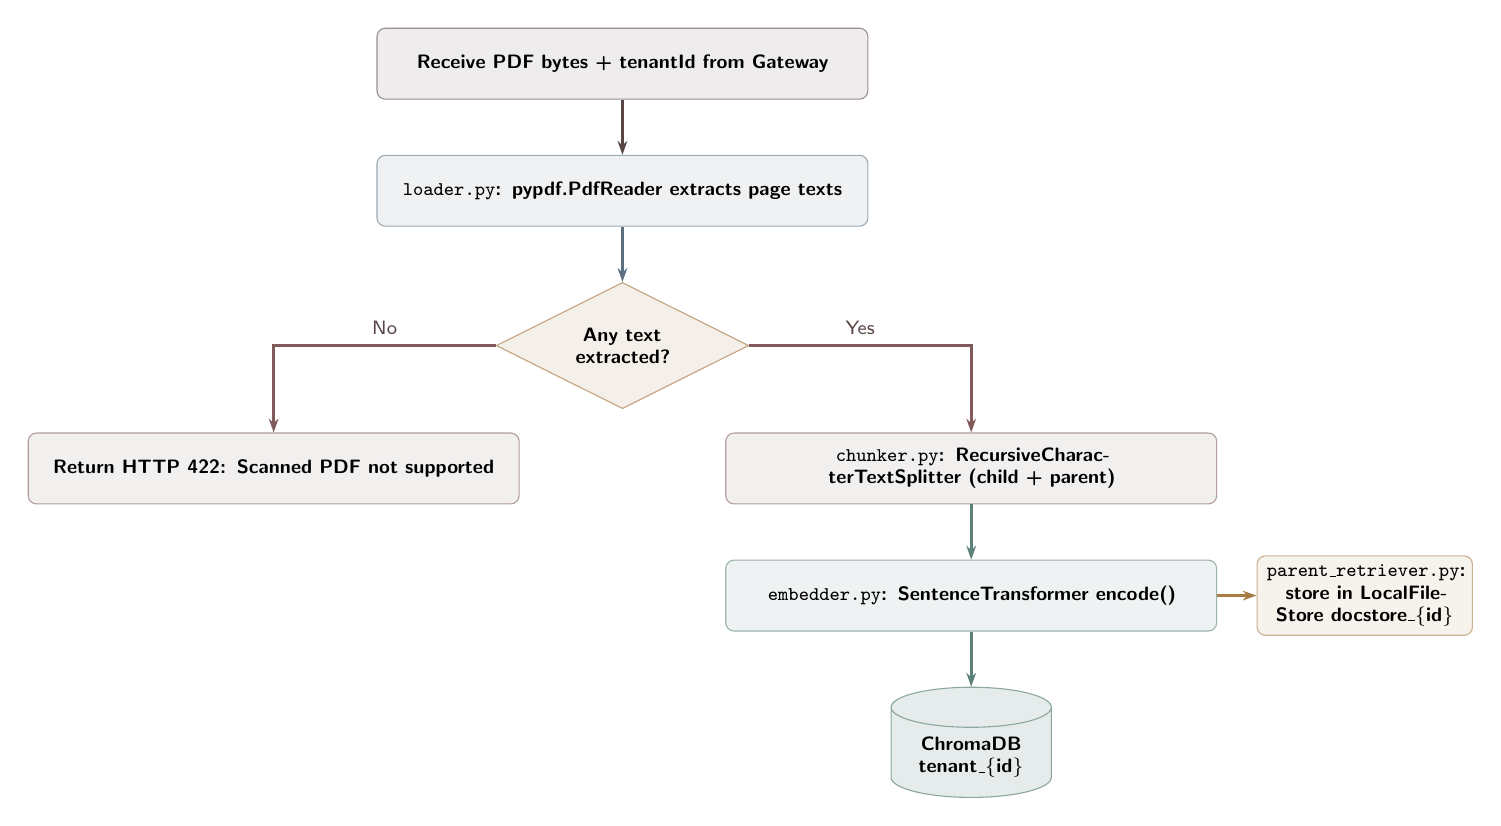
\begin{tikzpicture}[node distance=0.7cm]

  % Vertical main flow
  \node[proc=DarkEarth, text width=6cm] (recv)   {Receive PDF bytes + tenantId from Gateway};
  \node[proc=ABlue,     text width=6cm, below=0.7cm of recv]  (load)   {\texttt{loader.py}: pypdf.PdfReader extracts page texts};
  \node[dec,                            below=0.7cm of load]  (empty)  {Any text\\extracted?};

  % Yes branch — continues down
  \node[proc=DeepRose,  text width=6cm, below right=0.7cm and 0.5cm of empty] (chunk)  {\texttt{chunker.py}: RecursiveCharacterTextSplitter (child + parent)};
  \node[proc=AMint,     text width=6cm, below=0.7cm of chunk]  (embed)  {\texttt{embedder.py}: SentenceTransformer encode()};
  \node[dbs=AMint,                      below=0.7cm of embed]  (chroma) {ChromaDB tenant\_\{id\}};

  % Parallel parent store
  \node[proc=AAmber,    text width=2.5cm, right=0.5cm of embed]  (parent) {\texttt{parent\_retriever.py}: store in LocalFileStore docstore\_\{id\}};

  % No branch
  \node[proc=DeepRose,  text width=6cm, below left=0.7cm and 0.5cm of empty] (reject) {Return HTTP 422: Scanned PDF not supported};

  \draw[arr=DarkEarth] (recv)  -- (load);
  \draw[arr=ABlue]     (load)  -- (empty);
  \draw[arr=DeepRose]  (empty.east) -| node[near start,above,lbl]{Yes} (chunk.north);
  \draw[arr=AMint]     (chunk) -- (embed);
  \draw[arr=AMint]     (embed) -- (chroma);
  \draw[arr=AAmber]    (embed.east) -- (parent.west);
  \draw[arr=DeepRose]  (empty.west) -| node[near start,above,lbl]{No}  (reject.north);

\end{tikzpicture}
\caption{Full document ingestion pipeline: PDF bytes to indexed vector storage.}
\label{fig:ingest_pipeline}
\end{figure}

\subsection{Stage 1 — PDF Text Extraction}

The \texttt{load\_pdf()} function wraps the incoming byte stream in a \texttt{BytesIO} object and passes it to \texttt{pypdf.PdfReader}. It iterates over every page, calling \texttt{page.extract\_text()}.

\textbf{Validation rules:}
\begin{itemize}
  \item If a page returns an empty string, a warning is logged (likely a scanned page).
  \item If \emph{all} pages are empty, a \texttt{ValueError} is raised and the file is rejected with HTTP~422.
  \item If \texttt{pypdf} cannot parse the file (corrupt PDF), a \texttt{PdfReadError} is caught and converted to a user-friendly error.
\end{itemize}

\begin{lstlisting}[language=Python, caption=Page metadata structure returned by loader.py]
{
  "content": "Full text of page N...",
  "metadata": {
    "filename": "employee_handbook.pdf",
    "total_pages": 42
  }
}
\end{lstlisting}

\subsection{Stage 2 — The Double Chunking Strategy}

A \textbf{single} chunking approach forces a compromise between search accuracy and answer quality. DokuMind eliminates this compromise with a \textbf{Parent-Child dual-chunking} strategy.

\begin{figure}[htbp]
\centering
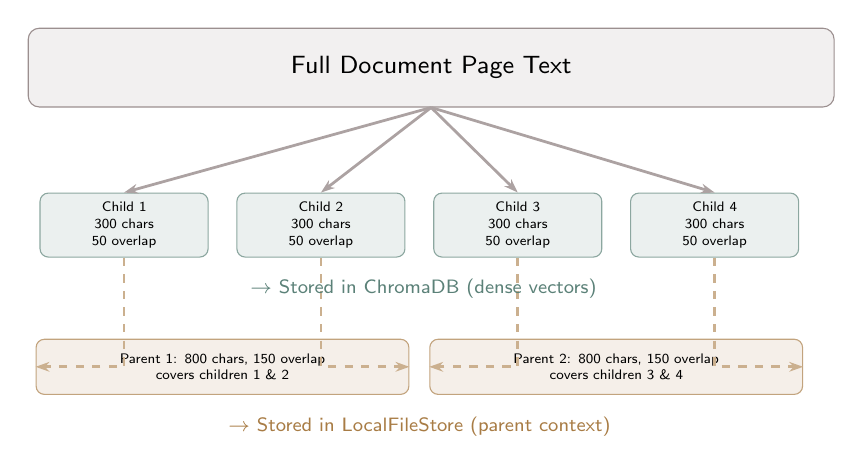
\begin{tikzpicture}

  % Source page text
  \node[draw=DarkEarth!60, fill=DarkEarth!8, rounded corners=4pt,
        text width=10cm, minimum height=1cm, align=center,
        font=\sffamily\small] (page) at (5,0) {Full Document Page Text};

  % Child chunks (row 1 — small)
  \foreach \i/\x in {1/1.1, 2/3.6, 3/6.1, 4/8.6}{
    \node[draw=AMint!70, fill=AMint!12, rounded corners=3pt,
          text width=1.9cm, minimum height=0.7cm, align=center,
          font=\sffamily\tiny] (c\i) at (\x, -2) {Child \i\\300 chars\\50 overlap};
    \draw[arr=DarkEarth!50] (page.south) -- (c\i.north);
  }

  % Parent chunks (row 2 — larger)
  \node[draw=AAmber!70, fill=AAmber!12, rounded corners=3pt,
        text width=4.5cm, minimum height=0.7cm, align=center,
        font=\sffamily\tiny] (p1) at (2.35, -3.8) {Parent 1: 800 chars, 150 overlap\\covers children 1 \& 2};
  \node[draw=AAmber!70, fill=AAmber!12, rounded corners=3pt,
        text width=4.5cm, minimum height=0.7cm, align=center,
        font=\sffamily\tiny] (p2) at (7.35, -3.8) {Parent 2: 800 chars, 150 overlap\\covers children 3 \& 4};

  \draw[arr=AAmber!60,dashed] (c1.south) |- (p1.west);
  \draw[arr=AAmber!60,dashed] (c2.south) |- (p1.east);
  \draw[arr=AAmber!60,dashed] (c3.south) |- (p2.west);
  \draw[arr=AAmber!60,dashed] (c4.south) |- (p2.east);

  % Storage labels
  \node[font=\sffamily\scriptsize\color{AMint},   below=0.15cm of c2,  xshift=1.3cm] {$\to$ Stored in ChromaDB (dense vectors)};
  \node[font=\sffamily\scriptsize\color{AAmber},  below=0.15cm of p1,  xshift=2.5cm] {$\to$ Stored in LocalFileStore (parent context)};

\end{tikzpicture}
\caption{Parent-Child double chunking: small child chunks for vector search, large parent chunks for LLM context.}
\label{fig:double_chunk}
\end{figure}

\begin{itemize}
  \item \textbf{Child chunks} (300 chars, 50 overlap) are laser-focused. Their embedding vector captures a single atomic concept, maximising cosine similarity accuracy during search.
  \item \textbf{Parent chunks} (800 chars, 150 overlap) are broader. When the LLM reads them, it has the surrounding sentences needed to compose a fluent, complete answer.
\end{itemize}

\subsection{Stage 3 — Semantic Embedding}

The \texttt{paraphrase-multilingual-MiniLM-L12-v2} model was selected for:
\begin{itemize}
  \item \textbf{Multilingual support}: handles English, French, and Arabic simultaneously.
  \item \textbf{384-dimensional output}: excellent semantic fidelity with compact storage.
  \item \textbf{Local inference}: no data leaves the server — runs entirely on CPU.
\end{itemize}

ChromaDB collections use \texttt{hnsw:space = "cosine"} for cosine distance search.

\section{Chat Query Pipeline}

\begin{figure}[htbp]
\centering
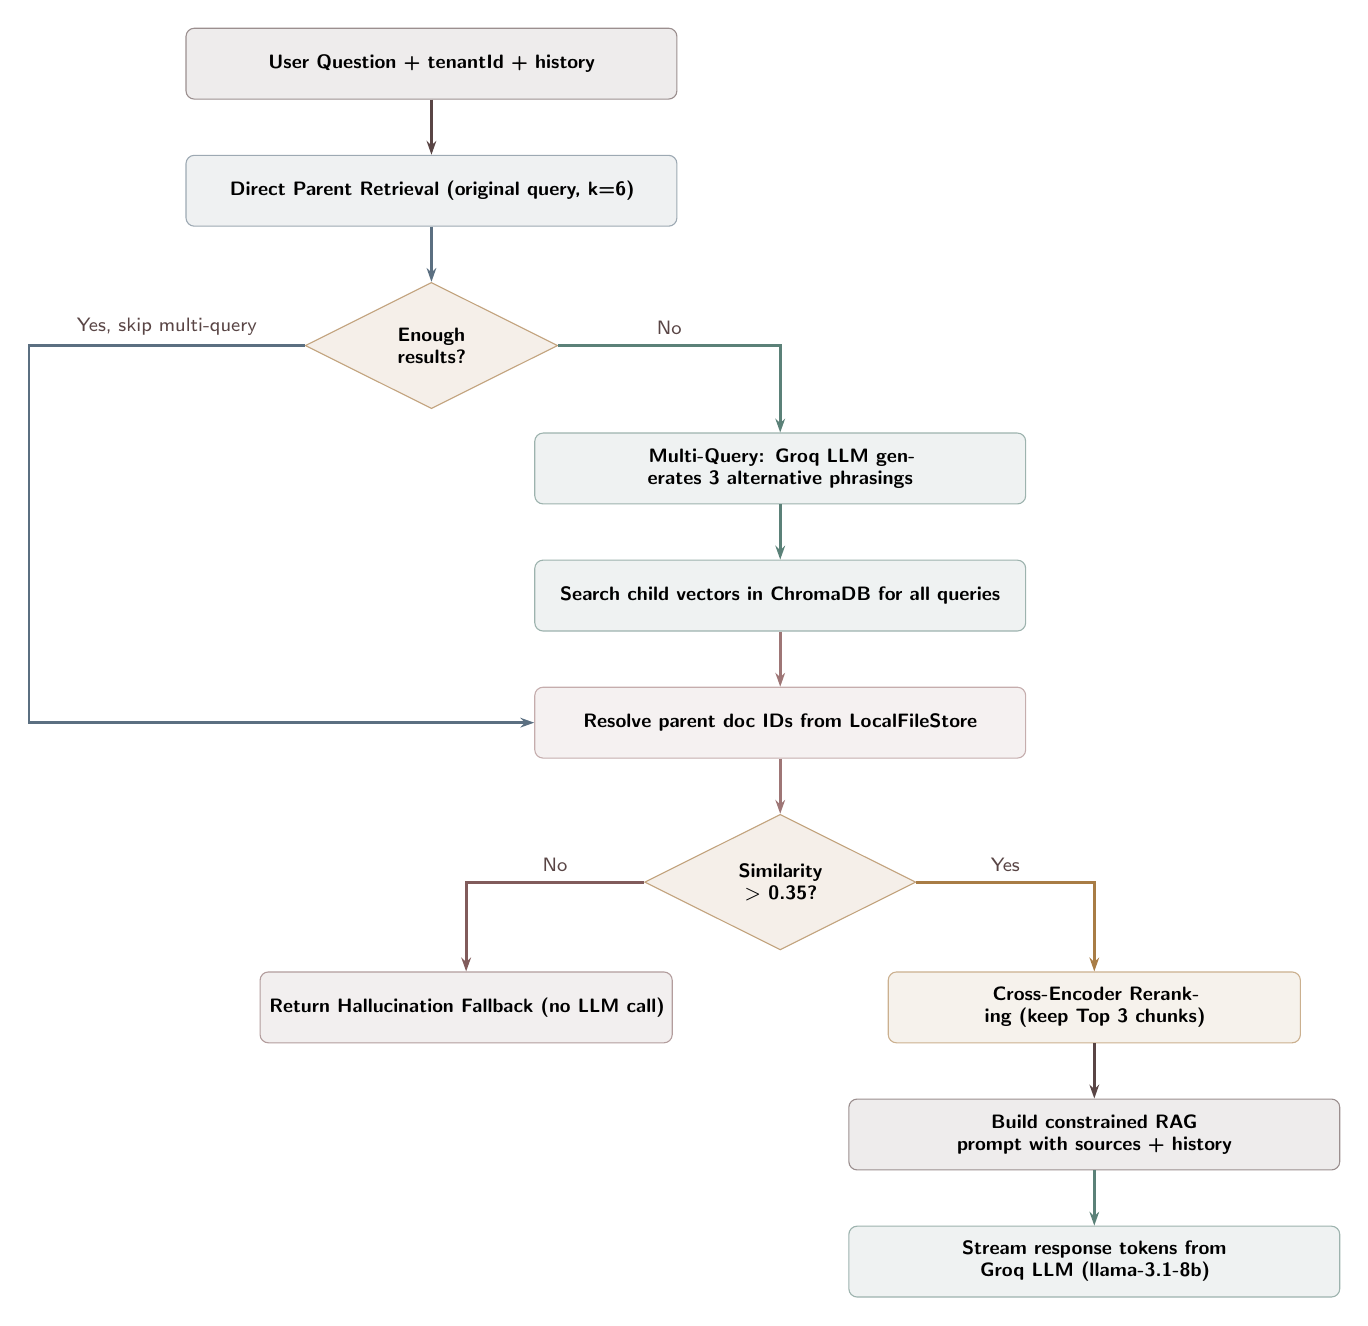
\begin{tikzpicture}[node distance=0.7cm]

  % Vertical flow — no horizontal sprawl
  \node[proc=DarkEarth, text width=6cm] (q)       {User Question + tenantId + history};
  \node[proc=ABlue,     text width=6cm, below=0.7cm of q]       (direct) {Direct Parent Retrieval (original query, k=6)};
  \node[dec,                            below=0.7cm of direct]  (enough) {Enough\\results?};

  % No branch — Multi-Query
  \node[proc=AMint,     text width=6cm, below right=0.7cm and 0.5cm of enough] (mq)     {Multi-Query: Groq LLM generates 3 alternative phrasings};
  \node[proc=AMint,     text width=6cm, below=0.7cm of mq]       (search) {Search child vectors in ChromaDB for all queries};
  \node[proc=MutedRose, text width=6cm, below=0.7cm of search]   (resolve){Resolve parent doc IDs from LocalFileStore};

  % Yes branch joins here
  \node[dec,            text width=1.8cm,below=0.7cm of resolve] (gate)   {Similarity\\$>$ 0.35?};

  \node[proc=DeepRose,  text width=5cm, below left=0.7cm and 0.5cm of gate]  (fallback){Return Hallucination Fallback (no LLM call)};
  \node[proc=AAmber,    text width=5cm, below right=0.7cm and 0.5cm of gate] (rerank)  {Cross-Encoder Reranking (keep Top 3 chunks)};
  \node[proc=DarkEarth, text width=6cm, below=0.7cm of rerank]   (prompt) {Build constrained RAG prompt with sources + history};
  \node[proc=AMint,     text width=6cm, below=0.7cm of prompt]   (groq)   {Stream response tokens from Groq LLM (llama-3.1-8b)};

  \draw[arr=DarkEarth] (q)       -- (direct);
  \draw[arr=ABlue]     (direct)  -- (enough);
  \draw[arr=AMint]     (enough.east) -| node[near start,above,lbl]{No}  (mq.north);
  \draw[arr=AMint]     (mq)      -- (search);
  \draw[arr=MutedRose] (search)  -- (resolve);
  \draw[arr=ABlue]     (enough.west) -| node[near start,above,lbl]{Yes, skip multi-query} ++(-3.5,0) |- (resolve.west);
  \draw[arr=MutedRose] (resolve) -- (gate);
  \draw[arr=DeepRose]  (gate.west)  -| node[near start,above,lbl]{No}  (fallback.north);
  \draw[arr=AAmber]    (gate.east)  -| node[near start,above,lbl]{Yes} (rerank.north);
  \draw[arr=DarkEarth] (rerank)  -- (prompt);
  \draw[arr=AMint]     (prompt)  -- (groq);

\end{tikzpicture}
\caption{Full chat query pipeline: from user question to streamed grounded response.}
\label{fig:chat_pipeline}
\end{figure}

\subsection{Multi-Query Expansion}

User queries are often short and ambiguous. The \texttt{search\_multi()} function first attempts a direct retrieval. If results are insufficient, it asks the Groq LLM to generate three alternative phrasings:

\begin{lstlisting}[language=Python, caption=Multi-Query expansion and query cleaning]
retriever = MultiQueryRetriever.from_llm(
    retriever=parent_retriever,
    llm=ChatGroq(model=settings.groq_model, temperature=0),
)
queries = retriever.llm_chain.invoke({"question": question})
# Strip numbered prefixes: "1. ", "2) ", etc.
cleaned = [re.sub(r'^\d+[\.\)\s]+', '', q).strip()
           for q in queries if q.strip()]
\end{lstlisting}

All variations are searched, results are aggregated with deduplication, and parent documents are resolved via the \texttt{LocalFileStore}.

\subsection{Cross-Encoder Reranking}

Cosine similarity (Bi-Encoder) embeds query and document independently — fast but occasionally imprecise. The Cross-Encoder (\texttt{ms-marco-MiniLM-L-6-v2}) processes the \emph{concatenated} (query, document) pair simultaneously through the transformer attention layers, yielding a highly precise relevance score.

\begin{lstlisting}[language=Python, caption=Cross-Encoder scoring and top-k selection]
reranker = CrossEncoder("cross-encoder/ms-marco-MiniLM-L-6-v2")
pairs = [(question, chunk["content"]) for chunk in chunks]
scores = reranker.predict(pairs)
for chunk, score in zip(chunks, scores):
    chunk["reranker_score"] = float(score)
reranked = sorted(chunks,
                  key=lambda x: x["reranker_score"],
                  reverse=True)
return reranked[:settings.top_k_after_rerank]  # Top 3
\end{lstlisting}

\subsection{Hallucination Guard}

Before calling the Groq API, \texttt{should\_fallback()} checks for meaningful context. If the maximum similarity score is below $0.35$, the pipeline short-circuits and returns deterministically:

\begin{lstlisting}[language=Python, caption=Deterministic hallucination protection]
FALLBACK = (
    "I don't have information on this topic in your "
    "company's documents. Please check with your HR "
    "department or consult the relevant policy directly."
)

def should_fallback(chunks: list) -> bool:
    return len(chunks) == 0
\end{lstlisting}

This is a \textbf{code-level guarantee} — not a prompt instruction. The LLM is never invoked if no valid evidence exists.

\subsection{Prompt Construction}

The \texttt{prompt\_builder.py} assembles the final prompt injecting retrieved contexts, source metadata, and conversation history into a strict template that instructs the LLM to answer only from provided passages.

% ==============================================================
% CHAPTER 6 — MULTI-TENANCY & SECURITY
% ==============================================================
\clearpage
\chapter{Multi-Tenancy \& Security Architecture}

\section{Tenant Isolation Across All Layers}

\begin{table}[htbp]
\centering
\caption{Tenant Isolation Strategy per Storage Layer}
\renewcommand{\arraystretch}{1.5}
\begin{tabularx}{\linewidth}{>{\bfseries\sffamily}l X X}
\toprule
\rowcolor{DeepRose!10}
Layer & Tenant A Scope & Tenant B Scope \\
\midrule
PostgreSQL   & \texttt{WHERE company\_id = UUID-A} & \texttt{WHERE company\_id = UUID-B} \\
MinIO        & \texttt{UUID-A/policy.pdf} & \texttt{UUID-B/policy.pdf} \\
ChromaDB     & Collection \texttt{tenant\_UUID-A} & Collection \texttt{tenant\_UUID-B} \\
LocalFileStore & \texttt{docstore\_UUID-A/} & \texttt{docstore\_UUID-B/} \\
\bottomrule
\end{tabularx}
\end{table}

\section{Security Hardening Measures}

\begin{itemize}
  \item \textbf{CORS}: Configured in \texttt{SecurityConfig} to allow only specific trusted origins.
  \item \textbf{HttpOnly Cookie}: Refresh tokens use \texttt{SameSite=Strict}, \texttt{HttpOnly=true}, scoped to \texttt{/auth/refresh} only.
  \item \textbf{BCrypt}: All passwords are hashed with BCrypt before any storage. Plain-text passwords are never persisted.
  \item \textbf{Dual JWT Secrets}: Access and Refresh tokens are signed with separate HMAC-SHA-256 secrets, so a stolen Access Token cannot forge a Refresh Token.
  \item \textbf{Tenant Validation}: The RAG Pipeline validates the \texttt{tenant\_id} format with a regex guard before executing any ChromaDB operation.
  \item \textbf{RBAC Constraints}: Service methods enforce hierarchical role rules server-side — frontend role checks are informational only.
\end{itemize}

% ==============================================================
% CHAPTER 7 — DOCKER & INFRASTRUCTURE
% ==============================================================
\clearpage
\chapter{Infrastructure \& Docker Deployment}

\section{Container Orchestration}

\begin{figure}[htbp]
\centering
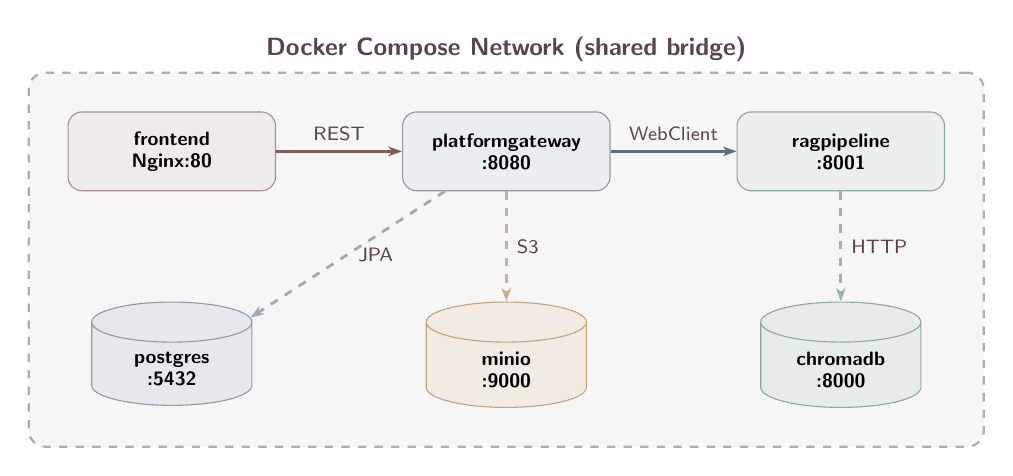
\begin{tikzpicture}[node distance=0.7cm]

  % Top row: user-facing services
  \node[svc=DeepRose] (fe)  {frontend\\Nginx:80};
  \node[svc=ABlue,  right=1.6cm of fe]  (gw)  {platformgateway\\:8080};
  \node[svc=AMint,  right=1.6cm of gw]  (rag) {ragpipeline\\:8001};

  % Bottom row: data stores
  \node[dbs=ABlue,  below=1.4cm of fe]  (pg)     {postgres\\:5432};
  \node[dbs=AAmber, below=1.4cm of gw]  (minio)  {minio\\:9000};
  \node[dbs=AMint,  below=1.4cm of rag] (chroma) {chromadb\\:8000};

  % Arrows
  \draw[arr=DeepRose]   (fe)  -- node[above,lbl]{REST}   (gw);
  \draw[arr=ABlue]      (gw)  -- node[above,lbl]{WebClient}(rag);
  \draw[arr=ABlue!60,dashed]  (gw)  -- node[right,lbl]{JPA}  (pg);
  \draw[arr=AAmber!60,dashed] (gw)  -- node[right,lbl]{S3}   (minio);
  \draw[arr=AMint!60,dashed]  (rag) -- node[right,lbl]{HTTP} (chroma);

  \begin{scope}[on background layer]
    \node[grp=DarkEarth, fit=(fe)(gw)(rag)(pg)(minio)(chroma), inner sep=14pt,
      label={[font=\sffamily\small\bfseries\color{DarkEarth}]above:Docker Compose Network (shared bridge)}] {};
  \end{scope}

\end{tikzpicture}
\caption{Docker Compose service graph: dependencies and inter-container communication.}
\label{fig:docker_compose}
\end{figure}

\section{Service-by-Service Configuration}

\begin{table}[htbp]
\centering
\caption{Docker Compose Service Specifications}
\renewcommand{\arraystretch}{1.4}
\begin{tabularx}{\linewidth}{>{\bfseries\sffamily}l l X}
\toprule
\rowcolor{DeepRose!10}
Service & Image / Build & Key Configuration \\
\midrule
postgres         & postgres:15             & healthcheck: pg\_isready; env: POSTGRES\_PASSWORD \\
minio            & minio/minio:latest      & healthcheck: curl /health/live; ports 9000 \& 9001 \\
chromadb         & chromadb/chroma:latest  & volume: ./chroma\_db\_data:/chroma/chroma \\
ragpipeline      & ./RAGPipeline (build)   & GROQ\_API\_KEY, CHROMA\_HOST; model weights cache volume \\
platformgateway  & ./PlatformGateway (build)& depends on postgres \& minio healthy; JWT secrets via env \\
frontend         & ./FrontEnd (build)      & VITE\_API\_URL build arg; Nginx port 80 \\
\bottomrule
\end{tabularx}
\end{table}

\subsection{Critical Volume Mounts}

\begin{itemize}
  \item \textbf{\texttt{./RAGPipeline/.cache:/root/.cache}} — Caches HuggingFace model weights on the host. Without it, every \texttt{docker compose up --build} re-downloads $\approx$800\,MB of transformer weights.
  \item \textbf{\texttt{./RAGPipeline/chroma\_db:/app/chroma\_db}} — Persists the LocalFileStore parent document KV store across restarts.
  \item \textbf{ChromaDB volume} — Persists HNSW vector indexes built during ingestion.
\end{itemize}

\subsection{Multi-Stage Dockerfiles}

\begin{itemize}
  \item \textbf{Frontend}: Stage 1 runs \texttt{npm run build} in Node~22. Stage 2 copies \texttt{dist/} into \texttt{nginx:alpine}. Zero Node.js runtime in production image.
  \item \textbf{PlatformGateway}: Stage 1 caches Maven dependencies. Stage 2 builds the JAR. Stage 3 runs in \texttt{eclipse-temurin:21-jre-alpine} only — build tools discarded.
  \item \textbf{RAGPipeline}: \texttt{python:3.11-slim}, installs gcc (required for some native extensions), then \texttt{pip install -r requirements.txt}. Models are not baked into the image; they are lazily downloaded into the mounted cache volume.
\end{itemize}

% ==============================================================
% CHAPTER 8 — CONCLUSION & ROADMAP
% ==============================================================
\clearpage
\chapter{Conclusion \& Future Roadmap}

\section{Summary of Achievements}

DokuMind Enterprise successfully integrates five distinct technologies into a seamless, enterprise-grade SaaS product, demonstrating that AI-powered corporate knowledge management need not compromise on security, accuracy, or data sovereignty.

\begin{conceptbox}{Key Achievements}
\begin{itemize}[noitemsep]
  \item \textbf{Zero-hallucination architecture} — deterministic similarity gating, no LLM guesswork
  \item \textbf{Advanced RAG pipeline} — Parent/Child chunking + Multi-Query + Cross-Encoder reranking
  \item \textbf{Complete multi-tenancy} — isolated at DB, object store, and vector store levels
  \item \textbf{Dual-token security} — HttpOnly cookies, BCrypt, separate HMAC secrets
  \item \textbf{Real-time streaming} — Groq LLM $\to$ Spring WebFlux $\to$ React SSE, character by character
  \item \textbf{Production-grade infra} — Docker Compose, healthchecks, volume persistence
\end{itemize}
\end{conceptbox}

\section{Future Roadmap}

\begin{table}[htbp]
\centering
\caption{Planned Feature Roadmap}
\renewcommand{\arraystretch}{1.4}
\begin{tabularx}{\linewidth}{>{\bfseries\sffamily}l >{\itshape}l X}
\toprule
\rowcolor{DeepRose!10}
Feature & Priority & Description \\
\midrule
OCR Integration           & High   & Tesseract/PaddleOCR for scanned PDF processing \\
Multi-Format Ingestion    & High   & Support .docx, .md, .xlsx, .html \\
Hybrid BM25/Dense Search  & High   & Combine sparse keyword matching with vector search \\
Analytics Dashboard       & Medium & Most-asked questions, knowledge gap detection \\
Per-Document ACL          & Medium & Fine-grained document access per role \\
Audit Logs                & Medium & Full trail of who queried what and when \\
Self-Hosted LLM           & Low    & Ollama integration for air-gapped deployments \\
\bottomrule
\end{tabularx}
\end{table}

% ==============================================================
% ABBREVIATIONS & ACRONYMS
% ==============================================================
\clearpage
\chapter*{Abbreviations \& Acronyms}
\addcontentsline{toc}{chapter}{Abbreviations \& Acronyms}

\begin{table}[H]
\centering
\renewcommand{\arraystretch}{1.5}
\begin{tabularx}{\linewidth}{>{\bfseries\sffamily\color{DeepRose}}l X}
\toprule
\rowcolor{DarkEarth!10}
\textcolor{black}{Acronym} & \textcolor{black}{Definition} \\
\midrule
RAG & Retrieval-Augmented Generation \\
LLM & Large Language Model \\
JWT & JSON Web Token \\
API & Application Programming Interface \\
SSE & Server-Sent Events \\
RBAC & Role-Based Access Control \\
ACL & Access Control List \\
ORM & Object-Relational Mapping \\
JPA & Java Persistence API \\
HNSW & Hierarchical Navigable Small World (Vector Indexing) \\
CORS & Cross-Origin Resource Sharing \\
DTO & Data Transfer Object \\
\bottomrule
\end{tabularx}
\end{table}

% ==============================================================
% REFERENCES / WEBOGRAPHY
% ==============================================================
\clearpage
\chapter*{References \& Webography}
\addcontentsline{toc}{chapter}{References \& Webography}

\begin{enumerate}[label={[\arabic*]}, itemsep=8pt]
    \item \textbf{Spring Boot Documentation}, Pivotal Software. Available at: \url{https://spring.io/projects/spring-boot}
    \item \textbf{React 19 Documentation}, Meta Open Source. Available at: \url{https://react.dev/}
    \item \textbf{FastAPI Framework}, Sebastián Ramírez. Available at: \url{https://fastapi.tiangolo.com/}
    \item \textbf{LangChain Python Framework}, Harrison Chase. Available at: \url{https://python.langchain.com/}
    \item \textbf{ChromaDB — The AI-native open-source embedding database}. Available at: \url{https://www.trychroma.com/}
    \item \textbf{Groq Cloud API Documentation}, Groq Inc. Available at: \url{https://groq.com/}
    \item \textbf{MinIO Object Storage Documentation}, MinIO Inc. Available at: \url{https://min.io/}
    \item \textbf{PostgreSQL Documentation}, PostgreSQL Global Development Group. Available at: \url{https://www.postgresql.org/}
    \item \textbf{Tailwind CSS Documentation}, Tailwind Labs. Available at: \url{https://tailwindcss.com/}
    \item \textbf{Sentence Transformers: Multilingual Sentence Embeddings}, Nils Reimers et al. Available at: \url{https://www.sbert.net/}
\end{enumerate}

\end{document}

